\documentclass[3p]{elsarticle}

\usepackage[T1]{fontenc}
\usepackage[utf8]{inputenc}
\usepackage{lmodern}
\usepackage{siunitx}
\sisetup{
	input-symbols = {()},
	per-mode=symbol,
}
\usepackage{lineno}
\usepackage{xspace}
\usepackage[hidelinks]{hyperref}
\usepackage[version=3]{mhchem}
\usepackage{tikz}							%To draw figures
\usepackage{tikz-3dplot}						%To facilitate drawing 3d figures
\usepackage{cleveref}
\usepackage{pgfplots}
\usepackage[justification=centering]{caption}
\usepackage{booktabs}
\usepackage{microtype}
\usepackage{subcaption}
\usepackage[flushleft]{threeparttable}
\usepackage{physics}
\usepackage{colortbl}
\usepackage [autostyle, english = american]{csquotes}
\usepackage{geometry}

%\usepackage{xfrac}'
\pgfplotsset{compat=newest}					%Set the pgfplots version to the newest version
\usetikzlibrary{backgrounds,
	external,
	positioning,
	patterns,
	hobby,
	shapes.geometric,
	pgfplots.groupplots,
	intersections}
\tikzexternalize[prefix=External/]			%Path to externalize figures

\modulolinenumbers[1]

\setlength{\footskip}{50pt}


\DeclareSIUnit\atm{atm}
\newcommand{\mole}{mole\xspace}
\newcommand{\Mole}{Mole\xspace}
\newcommand{\mr}{\mathit{MR}}

\journal{RadCal User Guide}

%%%%%%%%%%%%%%%%%%%%%%%
%% Elsevier bibliography styles
%%%%%%%%%%%%%%%%%%%%%%%
%% To change the style, put a % in front of the second line of the current style and
%% remove the % from the second line of the style you would like to use.
%%%%%%%%%%%%%%%%%%%%%%%

%% Numbered
%\bibliographystyle{model1-num-names}

%% Numbered without titles
%\bibliographystyle{model1a-num-names}

%% Harvard
%\bibliographystyle{model2-names.bst}\biboptions{authoryear}

%% Vancouver numbered
%\usepackage{numcompress}\bibliographystyle{model3-num-names}

%% Vancouver name/year
%\usepackage{numcompress}\bibliographystyle{model4-names}\biboptions{authoryear}

%% APA style
%\bibliographystyle{model5-names}\biboptions{authoryear}

%% AMA style
%\usepackage{numcompress}\bibliographystyle{model6-num-names}

%% `Elsevier LaTeX' style
\bibliographystyle{elsarticle-num}
%%%%%%%%%%%%%%%%%%%%%%%

\begin{document}
	
	\begin{frontmatter}

\title{Modifying the Spectral Radiative Properties of Soot in RADCAL and FDS}

%\author{Elsevier}
%\address{Radarweg 29, Amsterdam}

%% or include affiliations in footnotes:
\author[aalto]{Hadi Bordbar}
\ead{hadi.bordbar@aalto.fi}


\cortext[mycorrespondingauthor]{Corresponding author}

\address[aalto]{Department of Civil Engineering, Aalto University, Rakentajanaukio 4a, Espoo, 02150, Finland}


\begin{abstract}
The spectral soot radiation model is modified by using the correlations of Change and Charalampopoulos \cite{ChangeCharalampopoulos1990} for soot  spectral complex index of refraction. The effect of the change in predictions of RadCal is investigated through several cases. 
\end{abstract}

\begin{keyword}
Soot Radiation\sep Spectral Thermal Radiation\sep complex index of refraction
\end{keyword}

\end{frontmatter}


\allowdisplaybreaks

\section{Theory and Description of Models}\label{Cap:Introduction}
The soot spectral absorption coefficient is known to have to have a linear relation to the wave number \cite{modest2013radiative}. Accordingly, the previous version of RadCal used the following equation to calculate the soot spectral absorption coefficient
\begin{equation}
{\bar \kappa _\omega } = c\,\omega \,{f_v}
\label{Eq: Contant_C_Kappa}
\end{equation}
The spectrally constant coefficient of \(c = 7.0\) was used and referenced to an old work of Dalzell and Sarofim \cite{Dalzell1969_soot}. However, the coefficient of \(c = 7.0\) was not mentioned in that reference. Moreover, some fuel dependent values of \(c\) was mentioned in other references \cite{cassol2014application, YAGI1961288}. However, the experimental measurements done by Change and  Charalampopoulos \cite{ChangeCharalampopoulos1990} proposed two simple correlations for the real (\(n_s\)) and imaginary (\(k_s\)) parts of the complex index of refraction of soot which account for their dependency to wavelength (or wavenumber) as:
\begin{equation}
n_s=1.811+0.1263 ln(\lambda)+0.027ln^2(\lambda)+0.0417ln^3(\lambda)
\label{Eq:n_lambda}	
\end{equation}
and
\begin{equation}
k_s=0.5821+0.1213 ln(\lambda)+0.2309ln^2(\lambda)-0.01ln^3(\lambda)
\label{Eq:k_lambda}	
\end{equation}

where \({\lambda [\mu m]}\) represents wavelength and is given as \(\lambda [\mu m] = {{10000} \mathord{\left/
		{\vphantom {{10000} \omega }} \right.
		\kern-\nulldelimiterspace} \omega }[c{m^{ - 1}}]\).
Using the complex index of refraction, one can obtain the C values assuming Rayleigh regime for a cloud of soot particles as \cite{modest2013radiative,ChangeCharalampopoulos1990}:

\begin{equation}
C_\eta=\frac{36\pi n_s k_s}{(n_s^2-k_s^2+2)^2+4\pi n_s^2 k_s^2}
\label{Eq:C_Omega}
\end{equation}

To obtain a reasonable constant  \(c\), one can define a Planck weighted \(c\) as:
\begin{equation}
{\bar c_p} = \frac{{\int\limits_\omega  {{c_\omega }{I_{b\omega }}d\omega } }}{{\int\limits_\omega  {{I_{b\omega }}d\omega } }}
\end{equation}

\cref{Fig: PlanckWeightedC} shows the Planck weighted mean (i.e. \(c_p\)) for various temperatures occur in combustion systems.

\begin{figure}[h!]
			\centering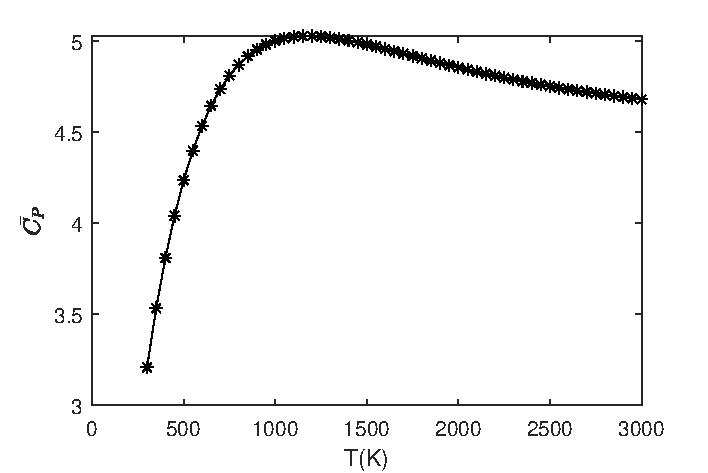
\includegraphics[width=12cm]{Figures/Fig1_P_C.pdf}
			\caption{How  Planck  mean  \({\bar c_p}\)  changes  with  temperature}
			\label{Fig: PlanckWeightedC}
\end{figure}
Considering \cref{Eq: Contant_C_Kappa}, another interesting average value to check can be defined as:
\begin{equation}
{\bar c_{p,\omega }} = \frac{{\int\limits_\omega  {{c_\omega }\omega {I_{b\omega }}d\omega } }}{{\int\limits_\omega  {\omega {I_{b\omega }}d\omega } }}
\end{equation}
\cref{Fig: PlanckWeightedCEta} shows \(\bar c_{p,\omega }\) for various temperatures occur in combustion systems.
  
\begin{figure}
	\centering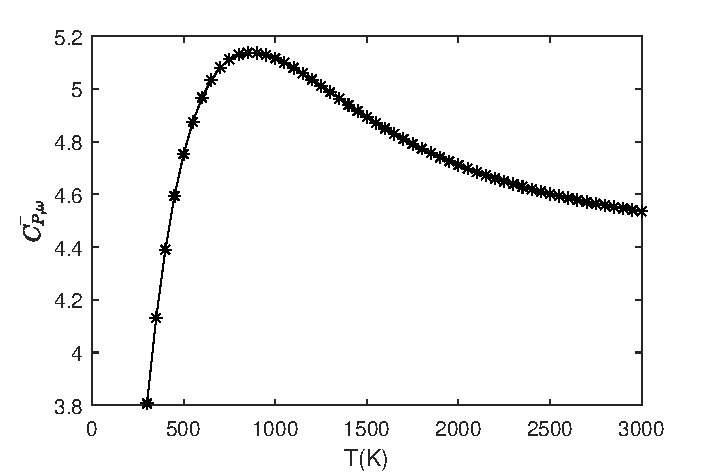
\includegraphics[width=12cm]{Figures/Fig2_P_C_eta.pdf}
	\caption{How  Planck  mean  \({\bar c_{p,\omega }}\)  changes  with  temperature}
	\label{Fig: PlanckWeightedCEta}
\end{figure}
Considering results shown in  \cref{Fig: PlanckWeightedC} and \cref{Fig: PlanckWeightedCEta}, it can be concluded that the constant \(c = 7.0\) may overestimate the role of soot radiation in overall thermal radiation of the systems. Alternatively, with a very small increment in computational time, we can directly calculate spectral  \(c_\omega\) using \cref{Eq:C_Omega} substuting the values of the spectral complex index of refraction calculated by the change and  Charalampopoulos \cite{ChangeCharalampopoulos1990} (i.e. \cref{Eq:n_lambda,Eq:k_lambda}).

\section{Results and Discussion}
In this section, the results of RadCal with the original soot radiation model (i.e. \cref{Eq: Contant_C_Kappa} with \(c = 7.0\)) are compared with those of using the modified model based on \cref{Eq:C_Omega,Eq:n_lambda,Eq:k_lambda}.

\subsection{Test Case 1: Cold Ethylene Layer}
In this test case a 31.75cm layer of Ethylene combustion products at T=300K located beside a wall at T=500K. The case is the same as the only example given in the current central repository of RadCal. The mole fraction of different species in the mixture is given as  \ce{C2H4} = 0.01 , \ce{CO2}= 0.0033, \ce{H2O}= 0.01, \ce{O2}= 0.21 , \ce{N2}= 0.7667, \(f_{v,soot}=10^{-7}\). To study the soot radiation contribution and the effect of the new modeling approach, this case is solved with various soot concentrations of \(f_{v,soot}=10^{-4}, 10^{-5}, 10^{-6}, 10^{-7}\), and \(10^{-8}\). This test case represents an absorption dominant scenario where the contribution of cold media in absorption of radiation coming from a hotter source (i,e, wall) is much larger than emission of the media. 
In the following figures of this section, the results of two different approaches of soot radiation modeling are compared for the test case 1.
For the very low soot concentration (e.g. \(f_{v,soot}=10^{-7}\) and \(10^{-8}\)), as seen in  \cref{fig:e_s8,fig:e_s7} the predictions of two models are quite the same as expected. In this condition the role of soot radiation is marginal and thermal radiation is governed by gas radiation mainly.


\begin{figure}[p]
	\centering\subfloat[The original soot model]{%
	\centering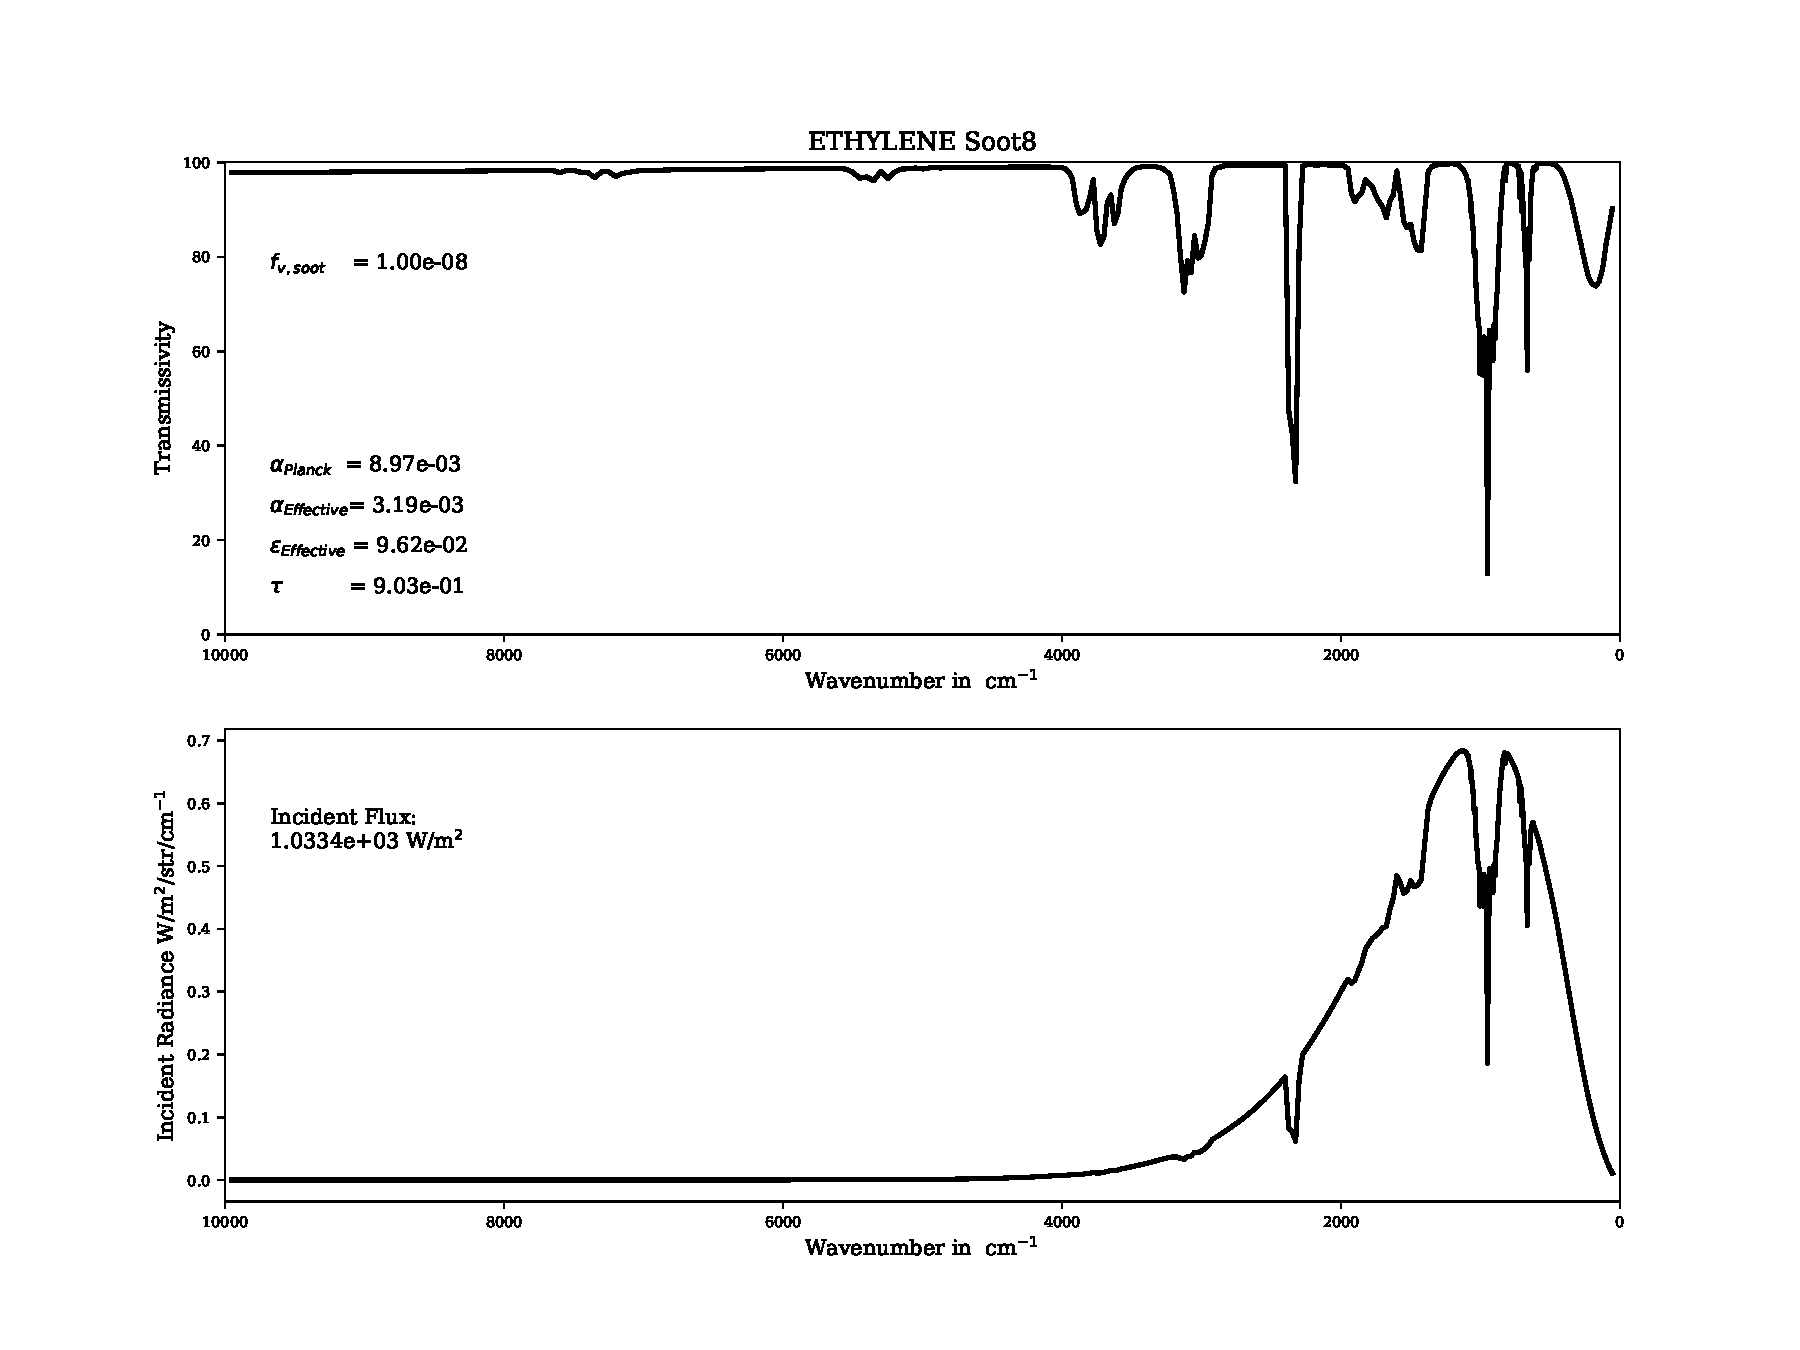
\includegraphics[width=14cm]{Figures/Cases_OriginalVersion (Soot C=7.0)/Tw500_Tg300_Ethylene_31cm/ETHYLENE_Soot8.pdf}%
	}
	\par\medskip
	\centering\subfloat[The modified soot model]{%
	\centering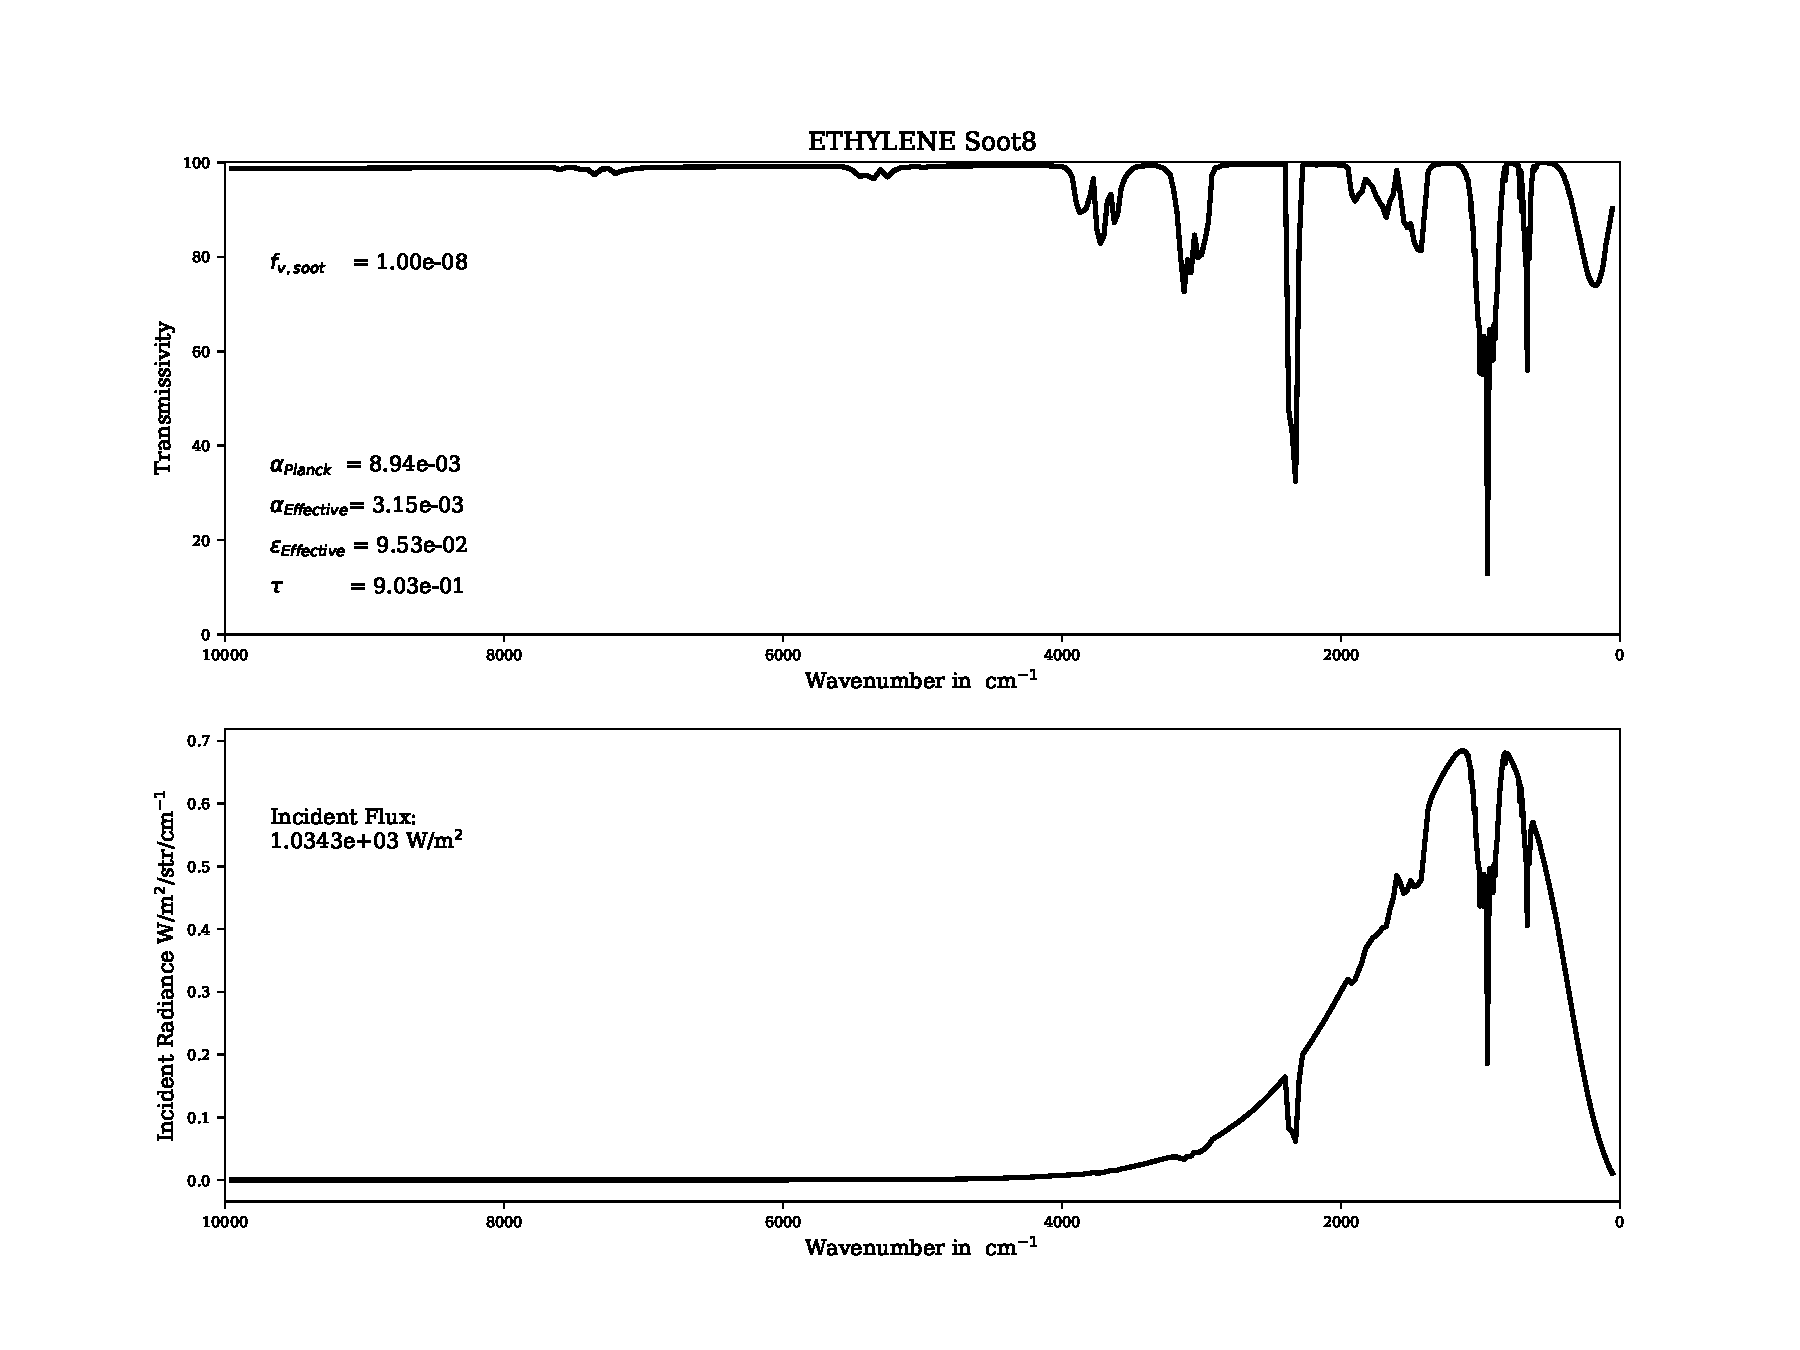
\includegraphics[width=14cm]{../Examples/Tw500_Tg300_Ethylene_31cm/Soot8/ETHYLENE_Soot8.pdf}%
	}
\caption{Test case 1, \({f_v=10^{-8}}\)} \label{fig:e_s8}
\end{figure}

\begin{figure}[hp]
	\centering\subfloat[The original soot model]{%
		\centering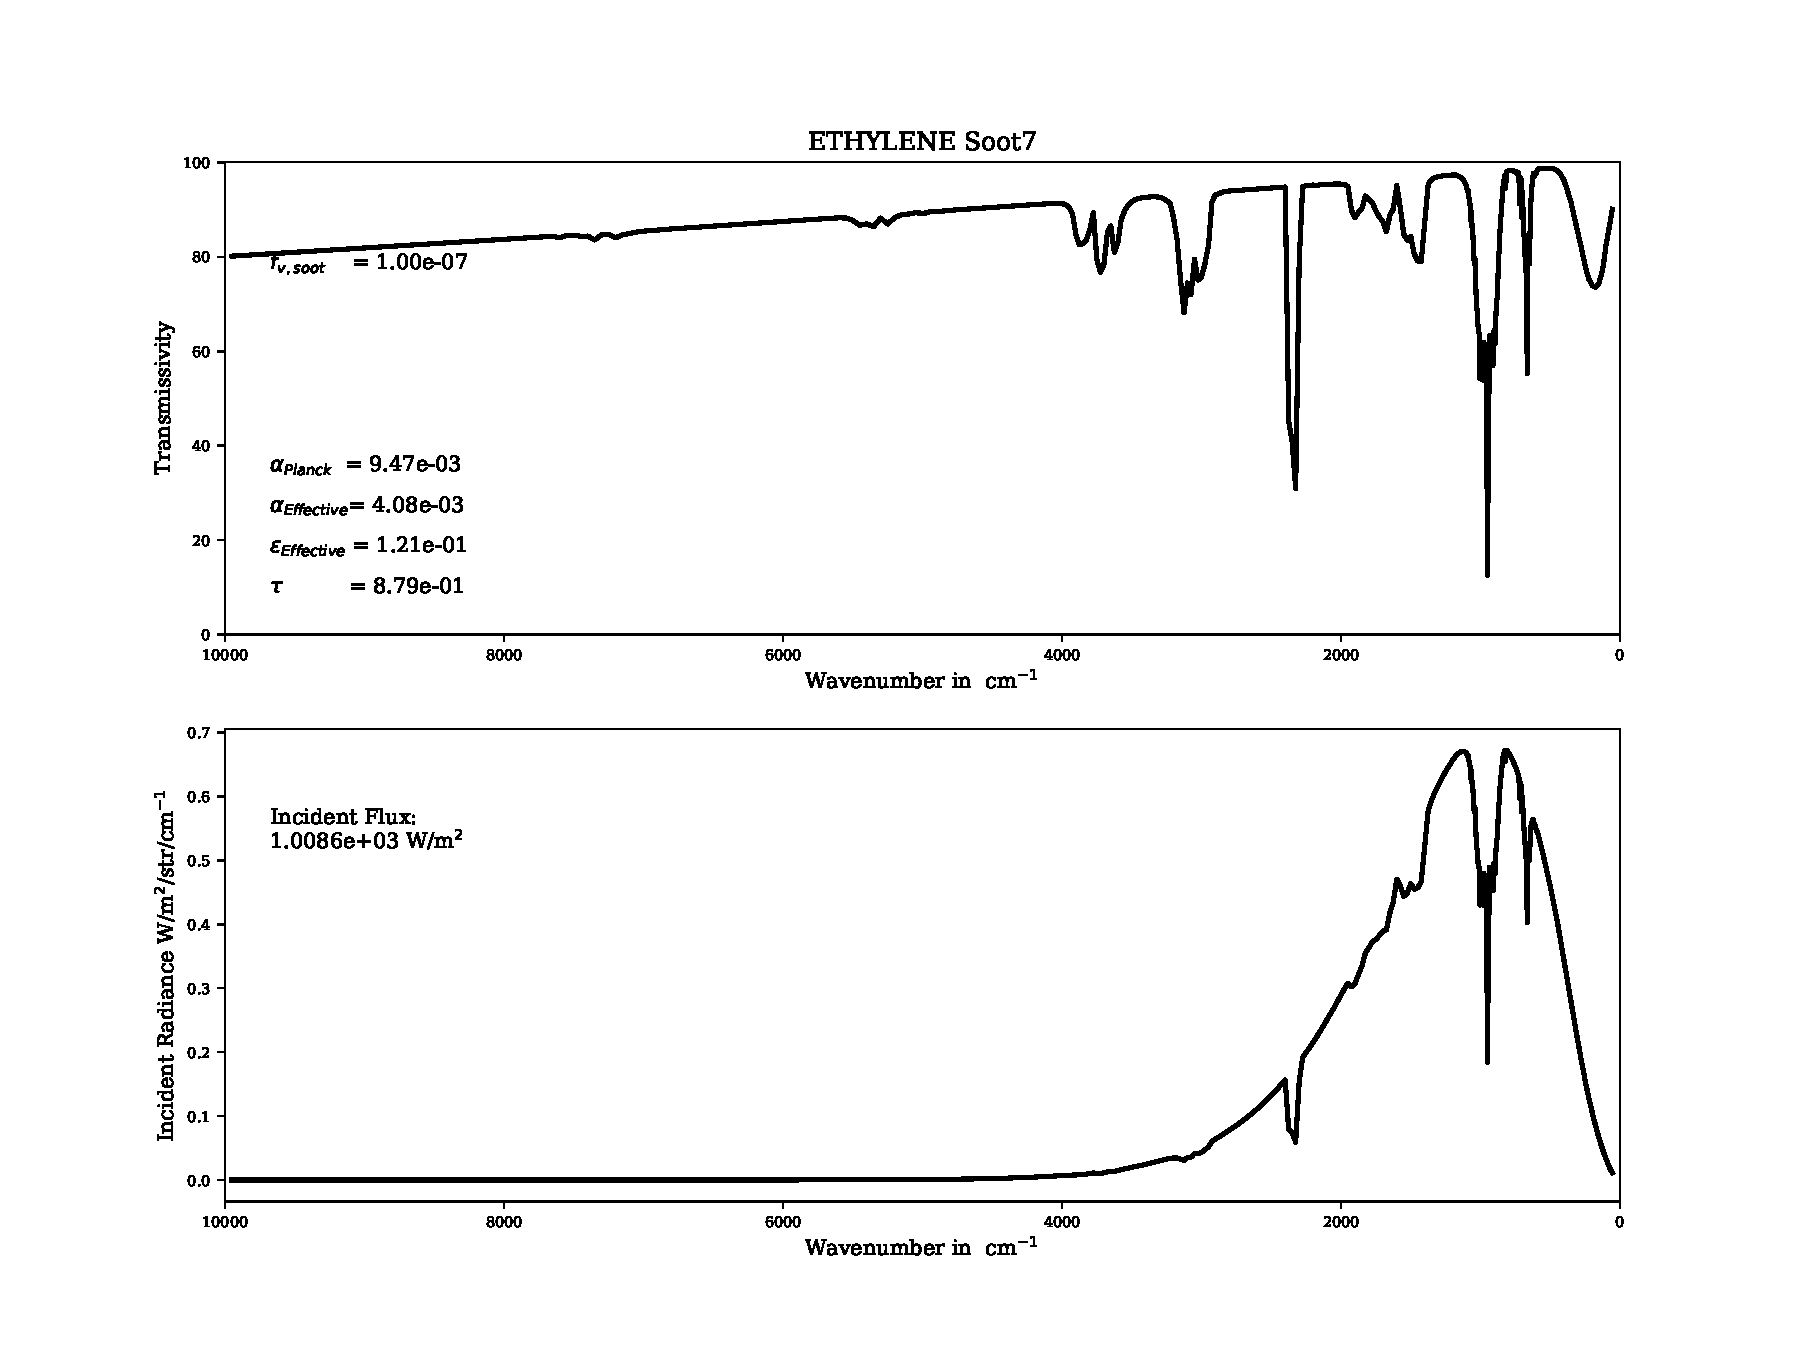
\includegraphics[width=14cm]{Figures/Cases_OriginalVersion (Soot C=7.0)/Tw500_Tg300_Ethylene_31cm/ETHYLENE_Soot7.pdf}%
	}
	\par\medskip		
	\centering\subfloat[The modified soot model]{%
		\centering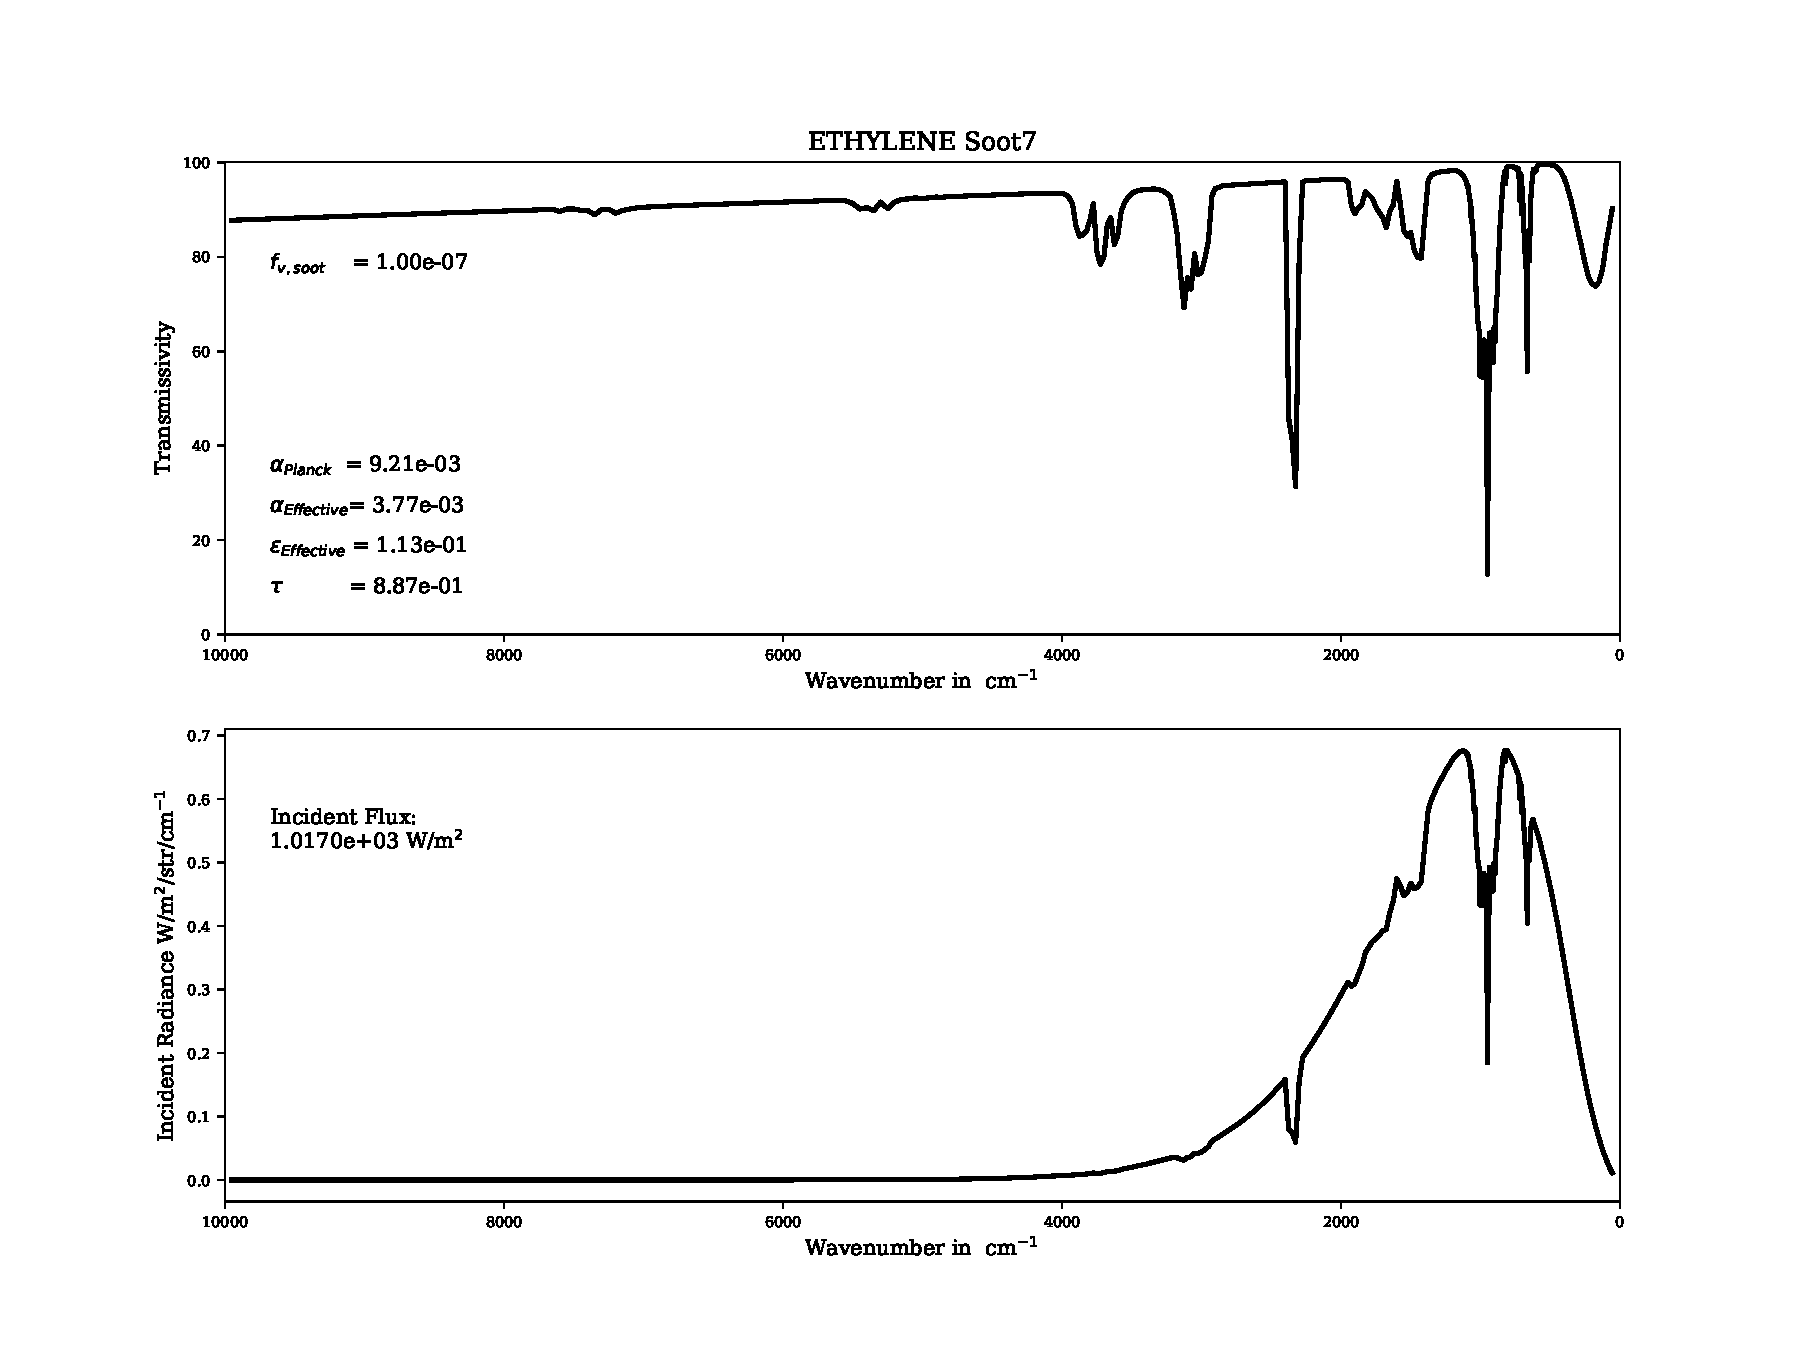
\includegraphics[width=14cm]{../Examples/Tw500_Tg300_Ethylene_31cm/Soot7/ETHYLENE_Soot7.pdf}%
	}
	\caption{Test case 1, \({f_v=10^{-7}}\)} \label{fig:e_s7}
\end{figure}
\pagebreak 
Similarly, for the cases with very large soot concentration (e.g. \(f_{v,soot}=10^{-4}\)), the proposed modification does not alter the results. For this high level of soot load, thermal radiation is governed by emission of soot and we see that the transmissivity is almost zero in the entire spectrum. It is also inline with theoretical expectations as in this concentration level, soot blocks the radiation and the whole mixture is acting like a blackbody emitter. It is seen for instance in the intensity profile of \cref{fig:e_s4} in which \(f_{v,soot}=10^{-4}\).

\begin{figure}[p]
	\centering\subfloat[The original soot model]{%
	\centering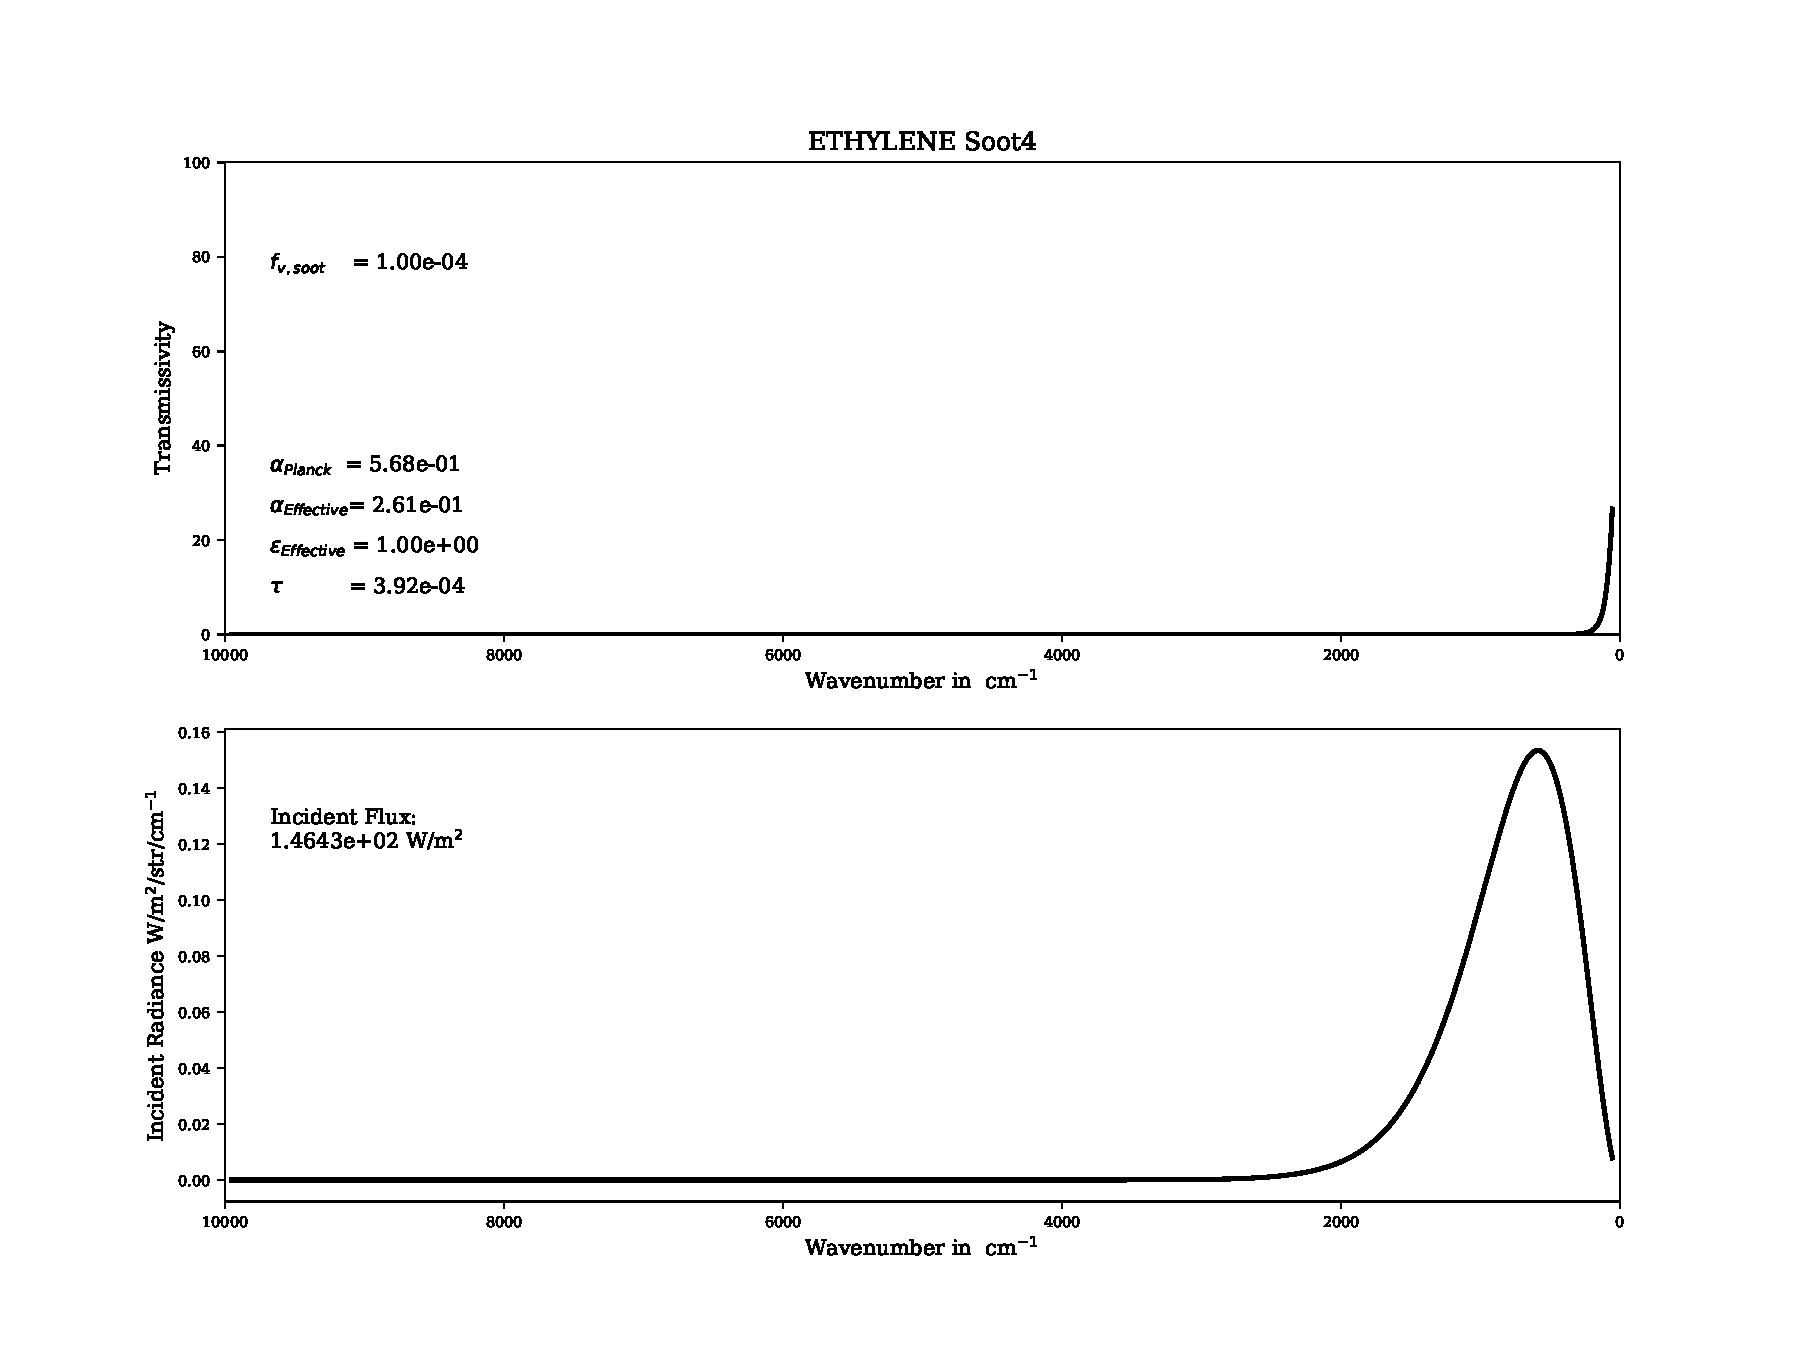
\includegraphics[width=14cm]{Figures/Cases_OriginalVersion (Soot C=7.0)/Tw500_Tg300_Ethylene_31cm/ETHYLENE_Soot4.pdf}%
	}
	\par\medskip		
	\centering\subfloat[The modified soot model]{%
		\centering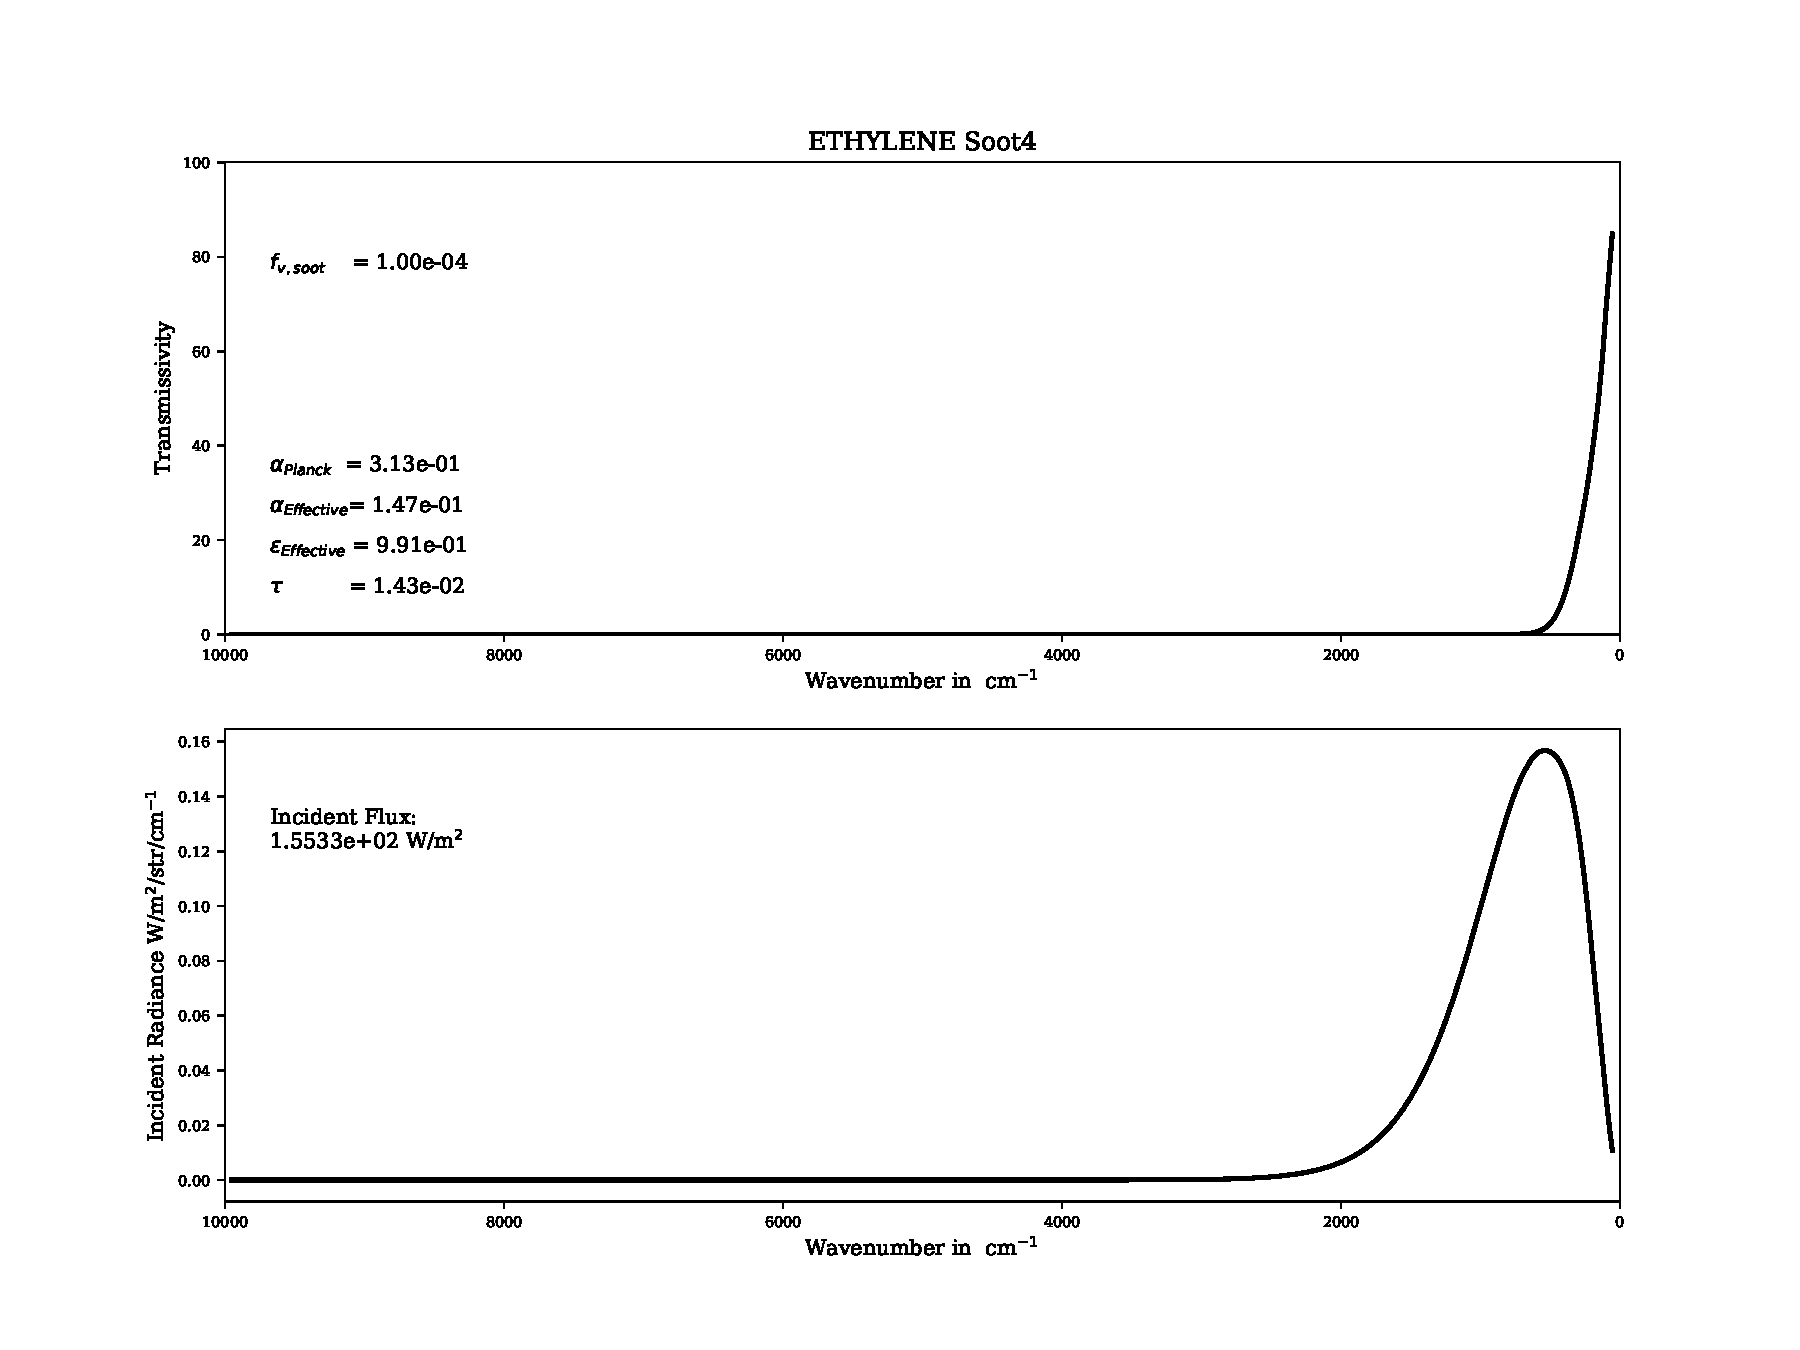
\includegraphics[width=14cm]{../Examples/Tw500_Tg300_Ethylene_31cm/Soot4/ETHYLENE_Soot4.pdf}%
	}
	\caption{Test case 1, \({f_v=10^{-4}}\)} \label{fig:e_s4}
\end{figure}

\pagebreak
 
However, for the moderate level of soot concentration (e.g. \(f_{v,soot}=10^{-5}\) and \(10^{-6}\)), quite remarkable differences are seen in predictions of two models for both profiles of transmissivity and intensity as seen in \cref{fig:e_s5,fig:e_s6}.The differences are more visible in low wavenumbers and total values.

\begin{figure}[p]
	\centering\subfloat[The original soot model]{%
		\centering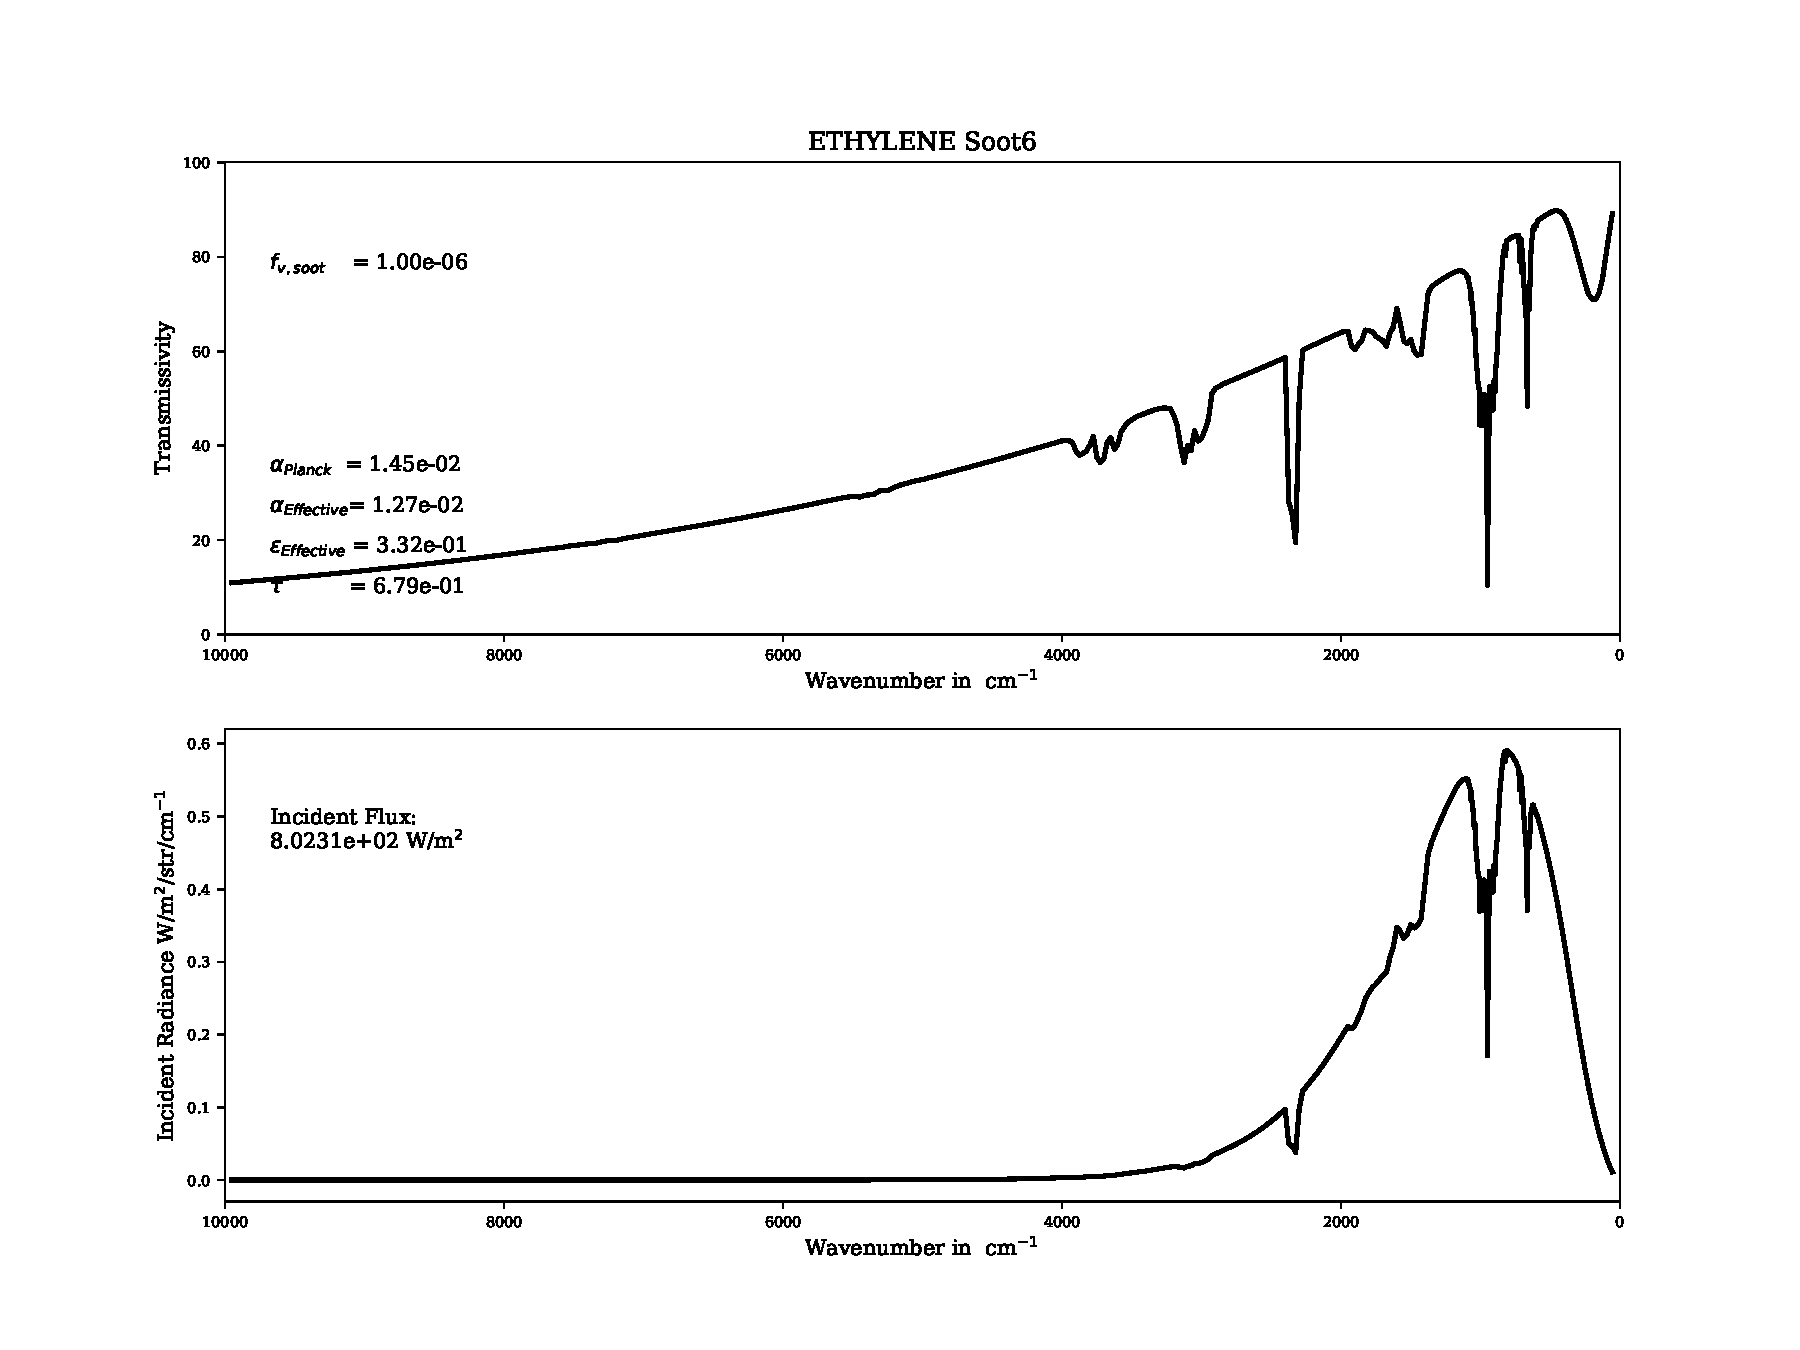
\includegraphics[width=14cm]{Figures/Cases_OriginalVersion (Soot C=7.0)/Tw500_Tg300_Ethylene_31cm/ETHYLENE_Soot6.pdf}%
	}
	\par\medskip		
	\centering\subfloat[The modified soot model]{%
		\centering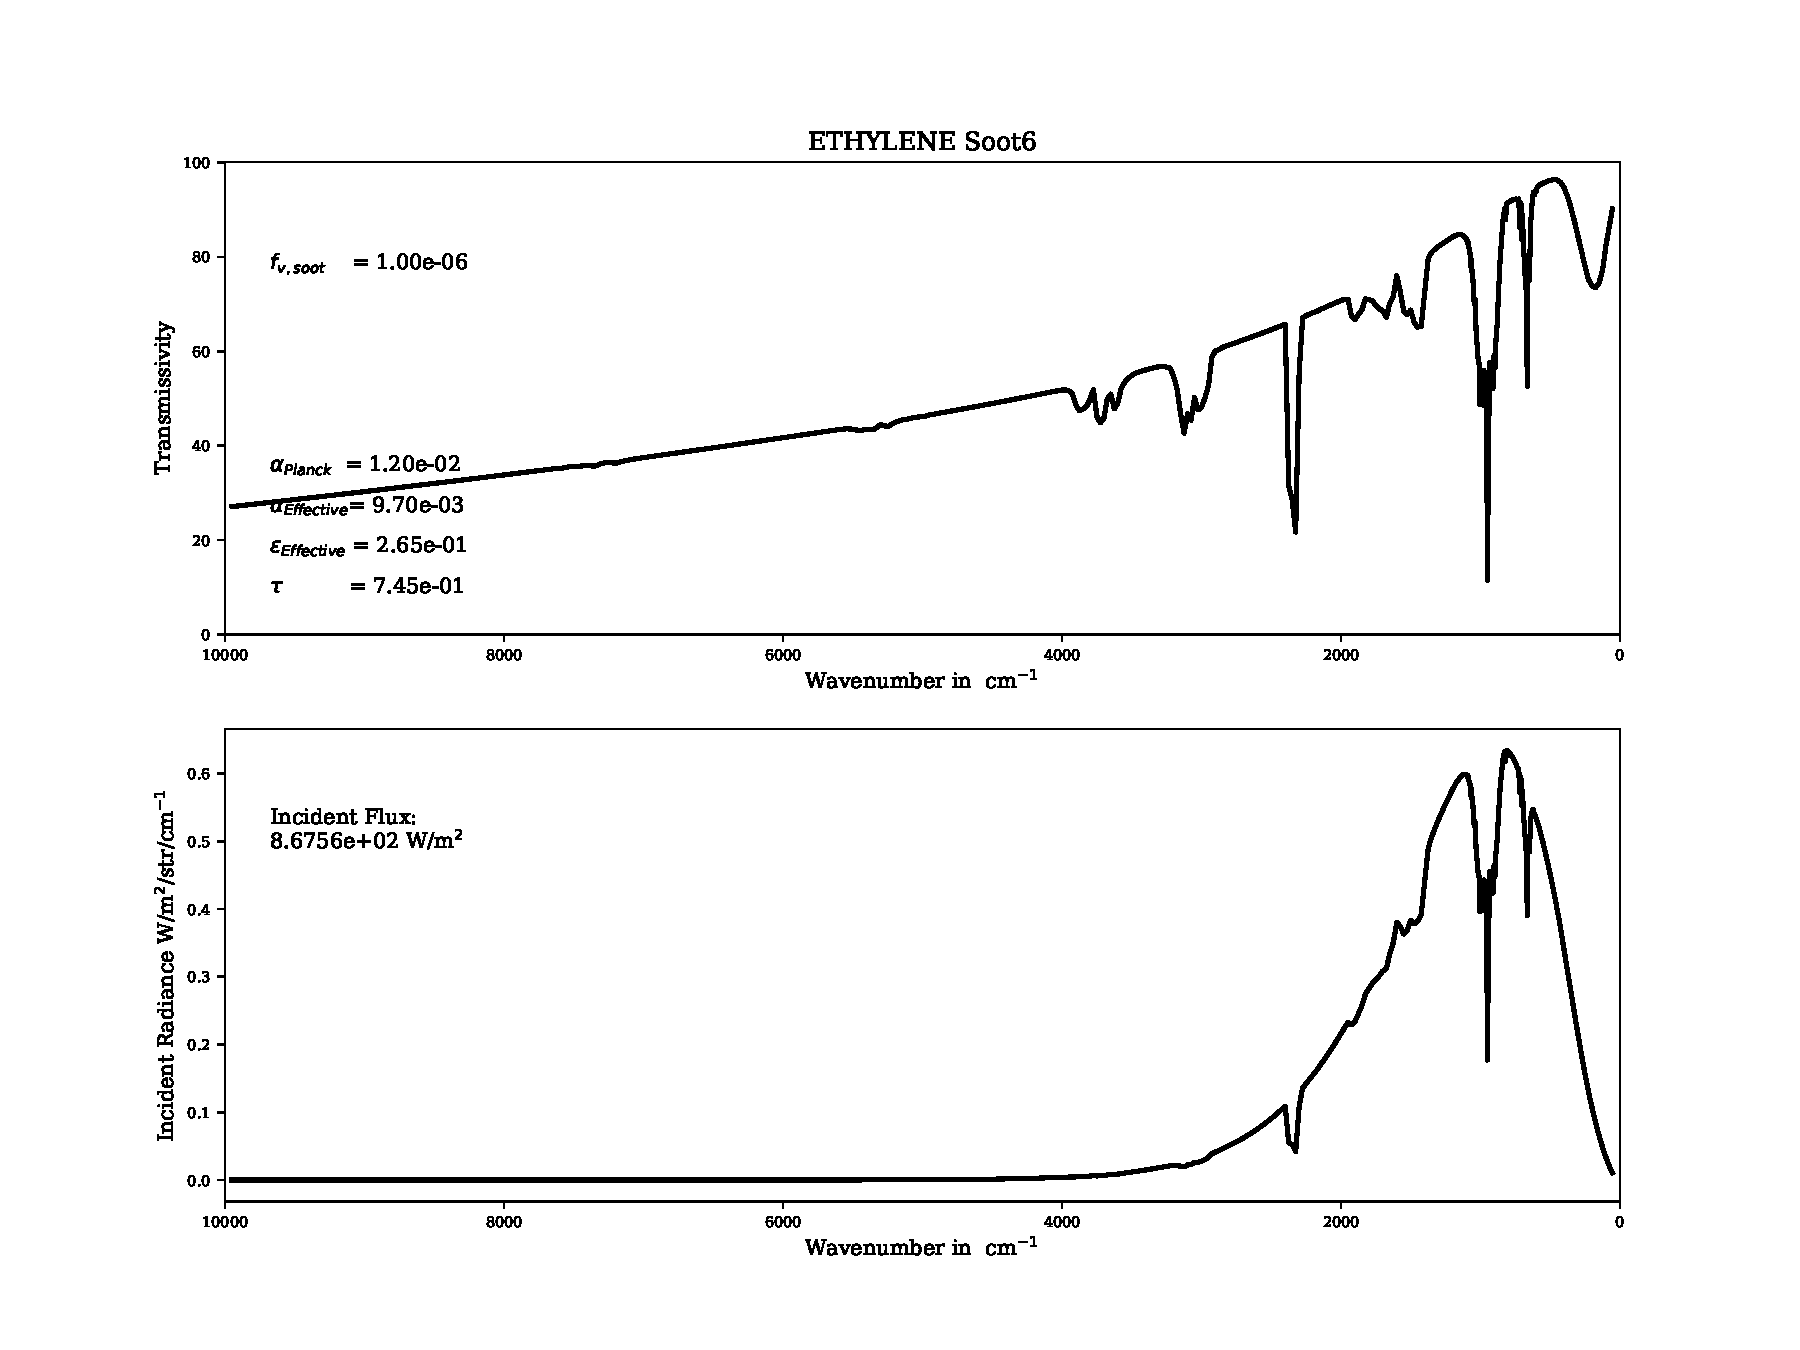
\includegraphics[width=14cm]{../Examples/Tw500_Tg300_Ethylene_31cm/Soot6/ETHYLENE_Soot6.pdf}%
	}
	\caption{Test case 1, \({f_v=10^{-6}}\)} \label{fig:e_s6}
\end{figure}


\begin{figure}[p]
	\centering\subfloat[The original soot model]{%
		\centering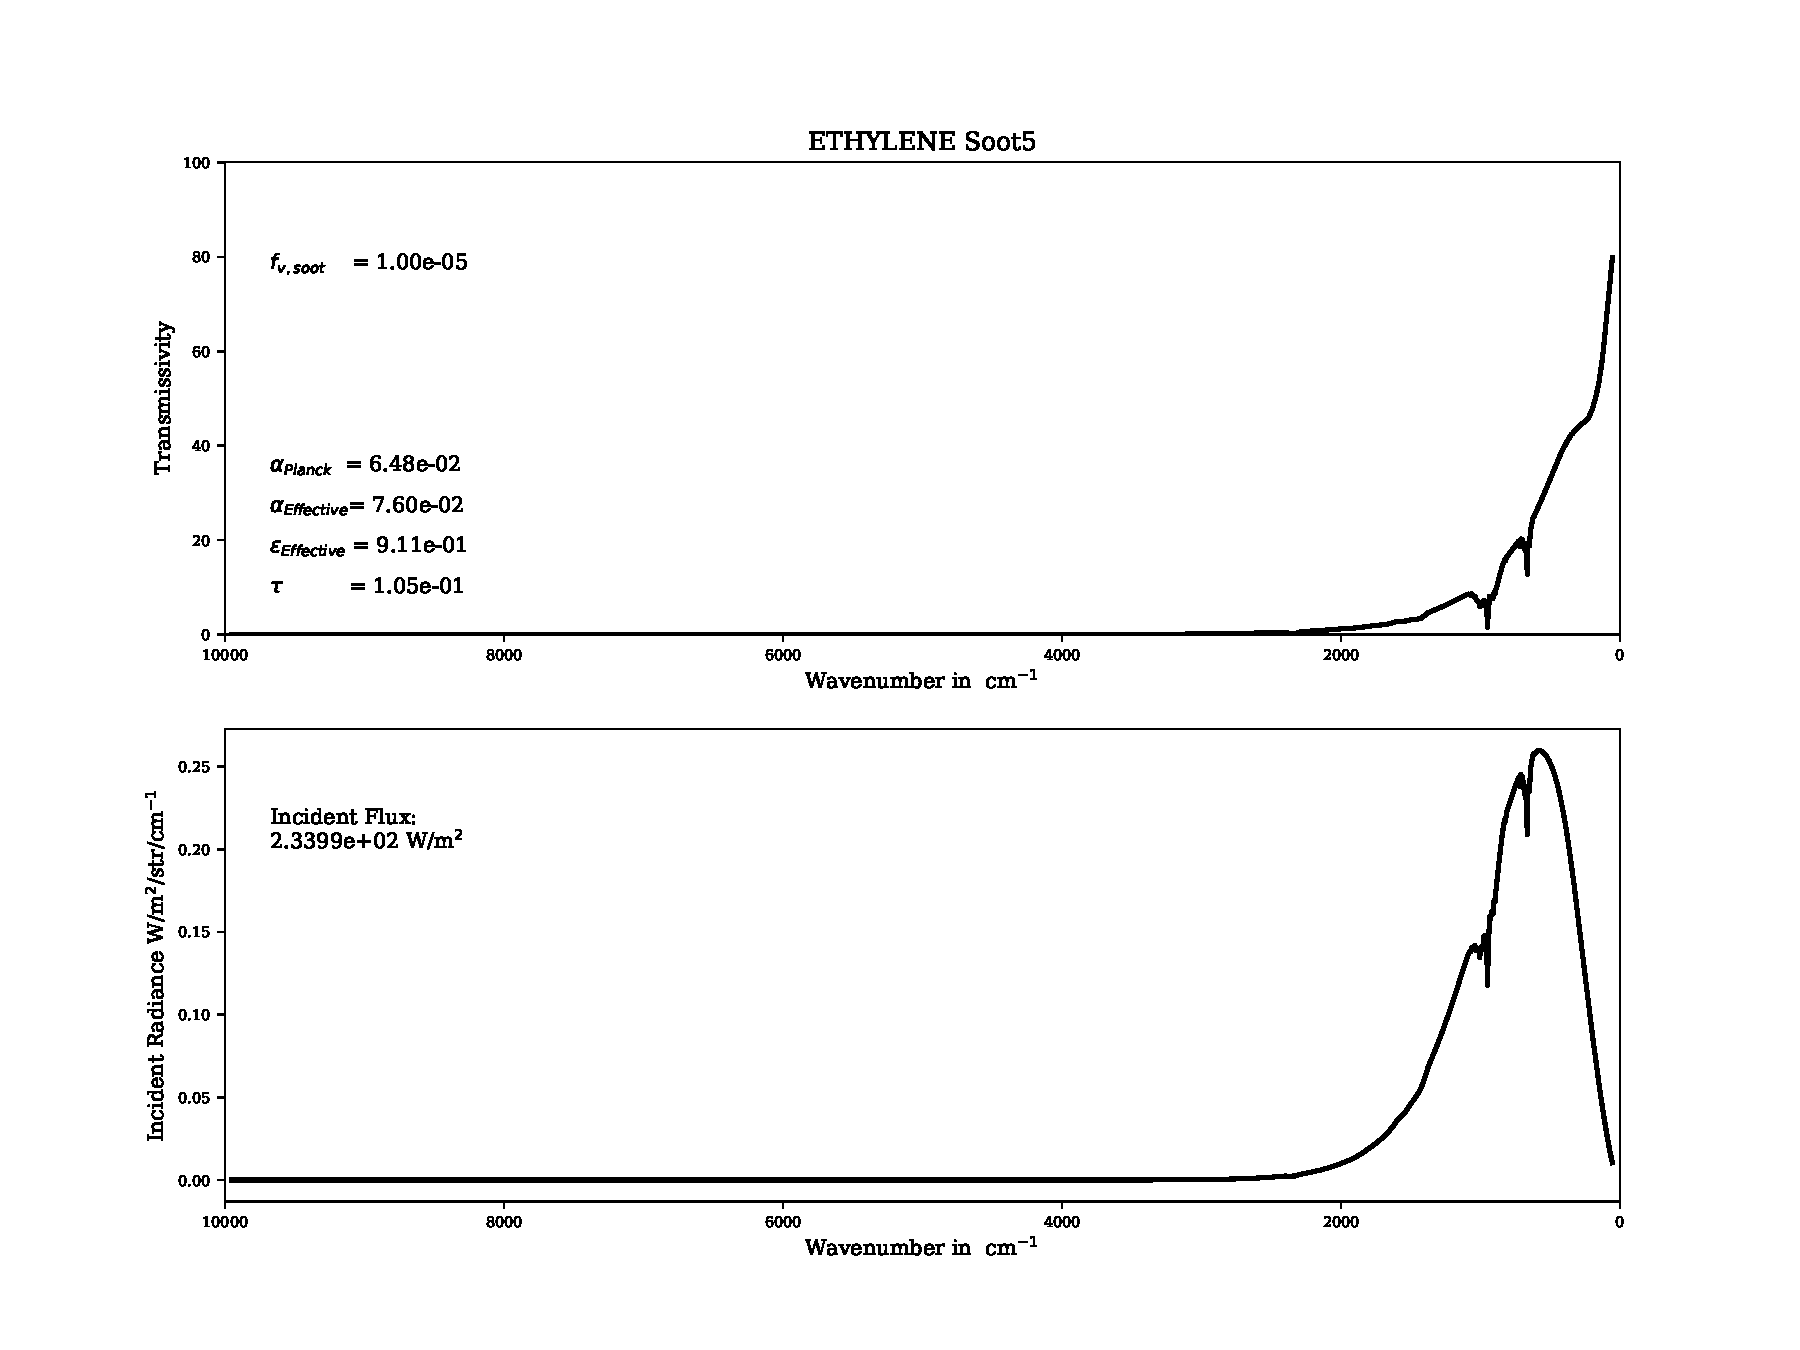
\includegraphics[width=14cm]{Figures/Cases_OriginalVersion (Soot C=7.0)/Tw500_Tg300_Ethylene_31cm/ETHYLENE_Soot5.pdf}%
	}
	\par\medskip		
	\centering\subfloat[The modified soot model]{%
		\centering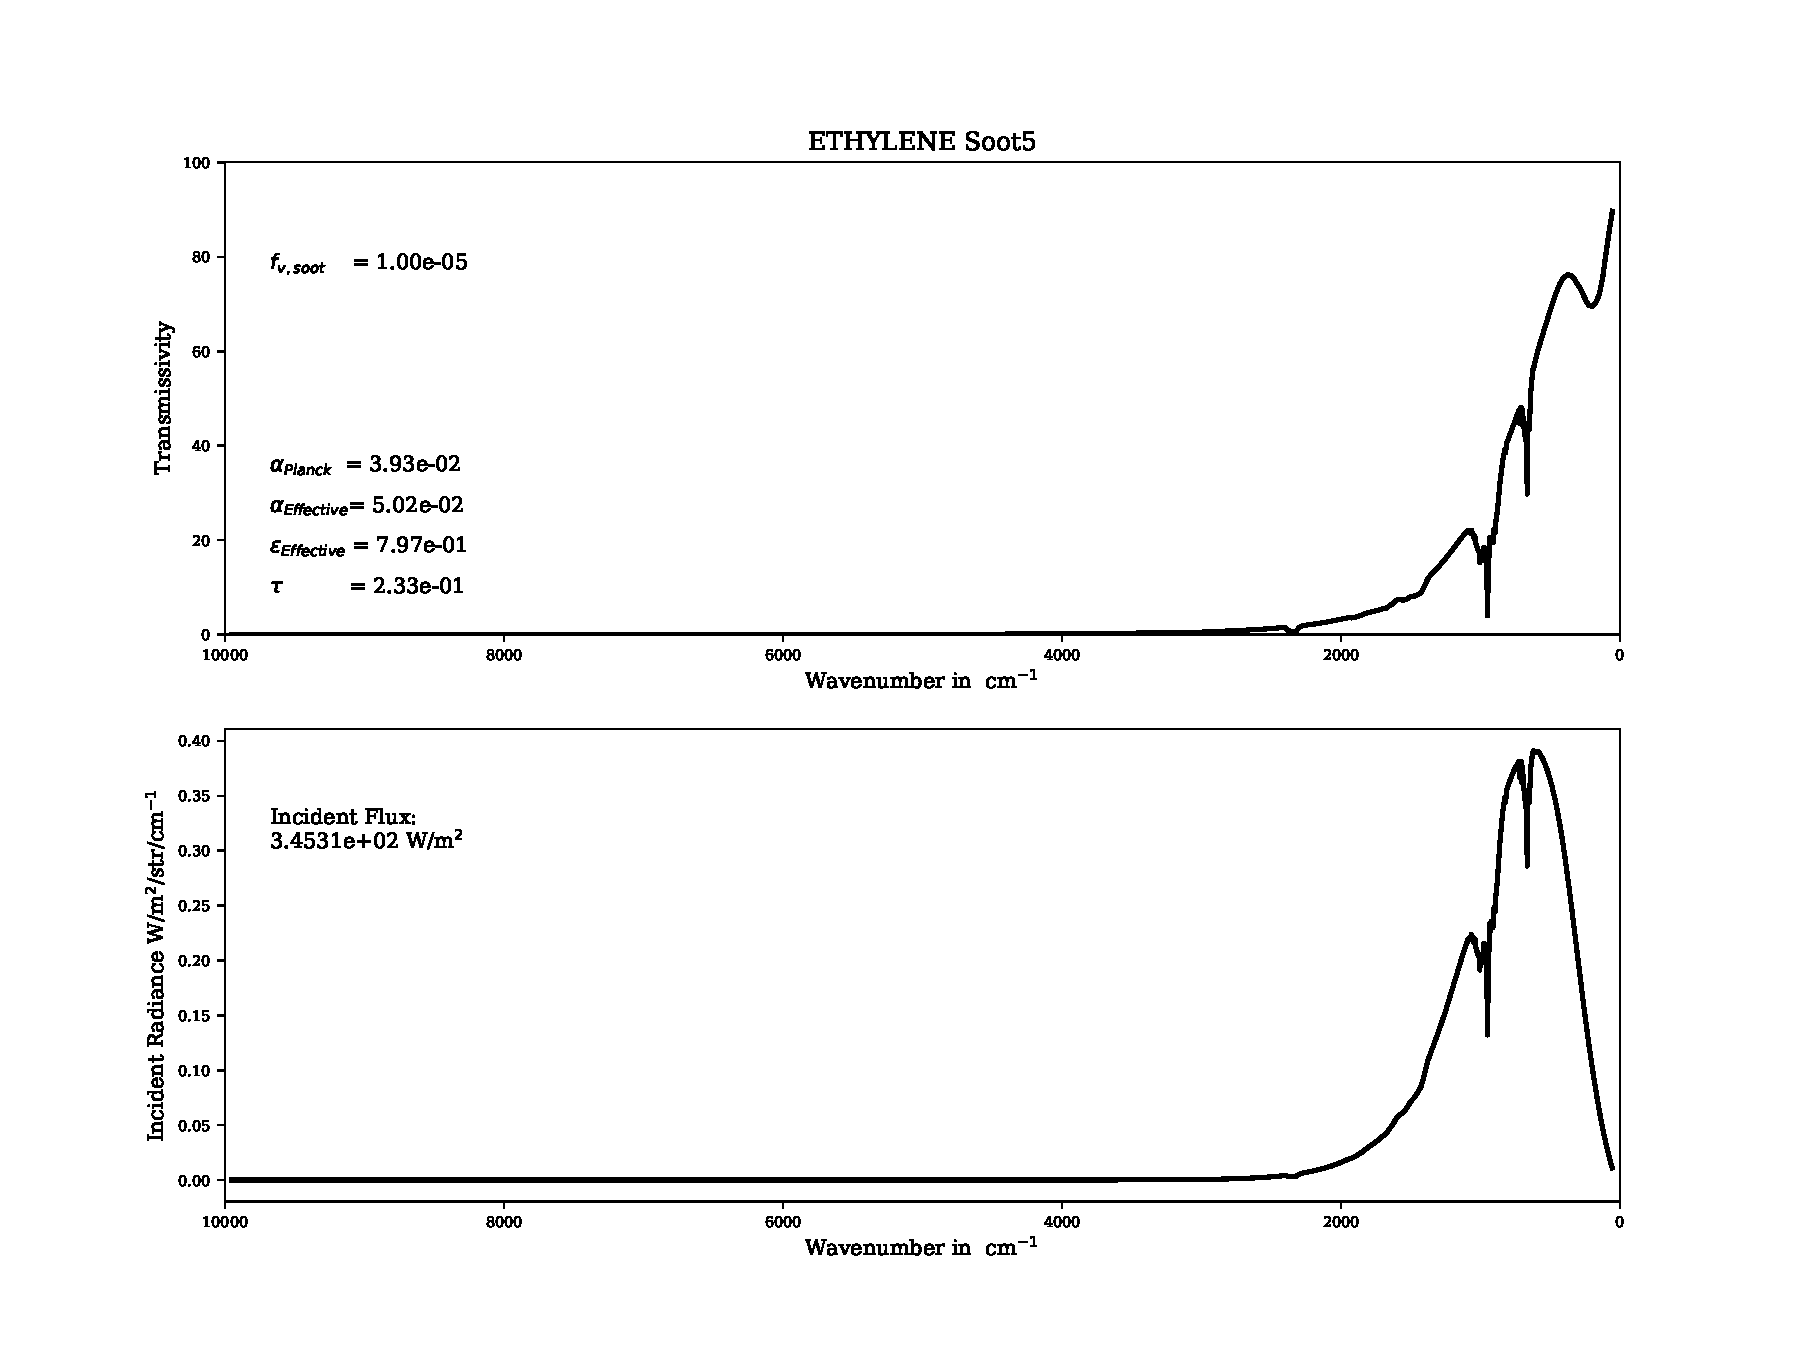
\includegraphics[width=14cm]{../Examples/Tw500_Tg300_Ethylene_31cm/Soot5/ETHYLENE_Soot5.pdf}%
	}
	\caption{Test case 1, \({f_v=10^{-5}}\)} \label{fig:e_s5}
\end{figure}

\pagebreak

\subsection{Test Case 2: Hot Methane Layer}
In this test case a 1m layer of Methane combustion products at T=1000K located beside a wall at T=300K.  The mole fraction of different gas species in the mixture is given as  \ce{CH4} = 0.0133 , \ce{CO2}= 0.07, \ce{H2O}= 0.14, \ce{O2}=0.01 , \ce{N2}= 0.7667. Similar to the previous case, this case is also solved with various soot concentrations of \(f_{v,soot}=10^{-4}, 10^{-5}, 10^{-6}, 10^{-7}\), and \(10^{-8}\). This test case represents an emission dominant scenario where the contribution of hot media in emission is much larger than their absorption of the source radiation(i.e. wall). 
In the following figures, the results of two different approaches of soot radiation modeling are compared for the test case 2.
For the very low soot concentration (e.g. \(f_{v,soot}=10^{-8}\) and \(10^{-7}\)), as seen in  \cref{fig:m_s8,fig:m_s7} the predictions of two models are quite the same as expected. In this condition the role of soot radiation is marginal and thermal radiation is governed by gas radiation mainly. However, small differences are seen in total values of intensity and mean absorption coefficients. 

\begin{figure}[p]
	\centering\subfloat[The original soot model]{%
		\centering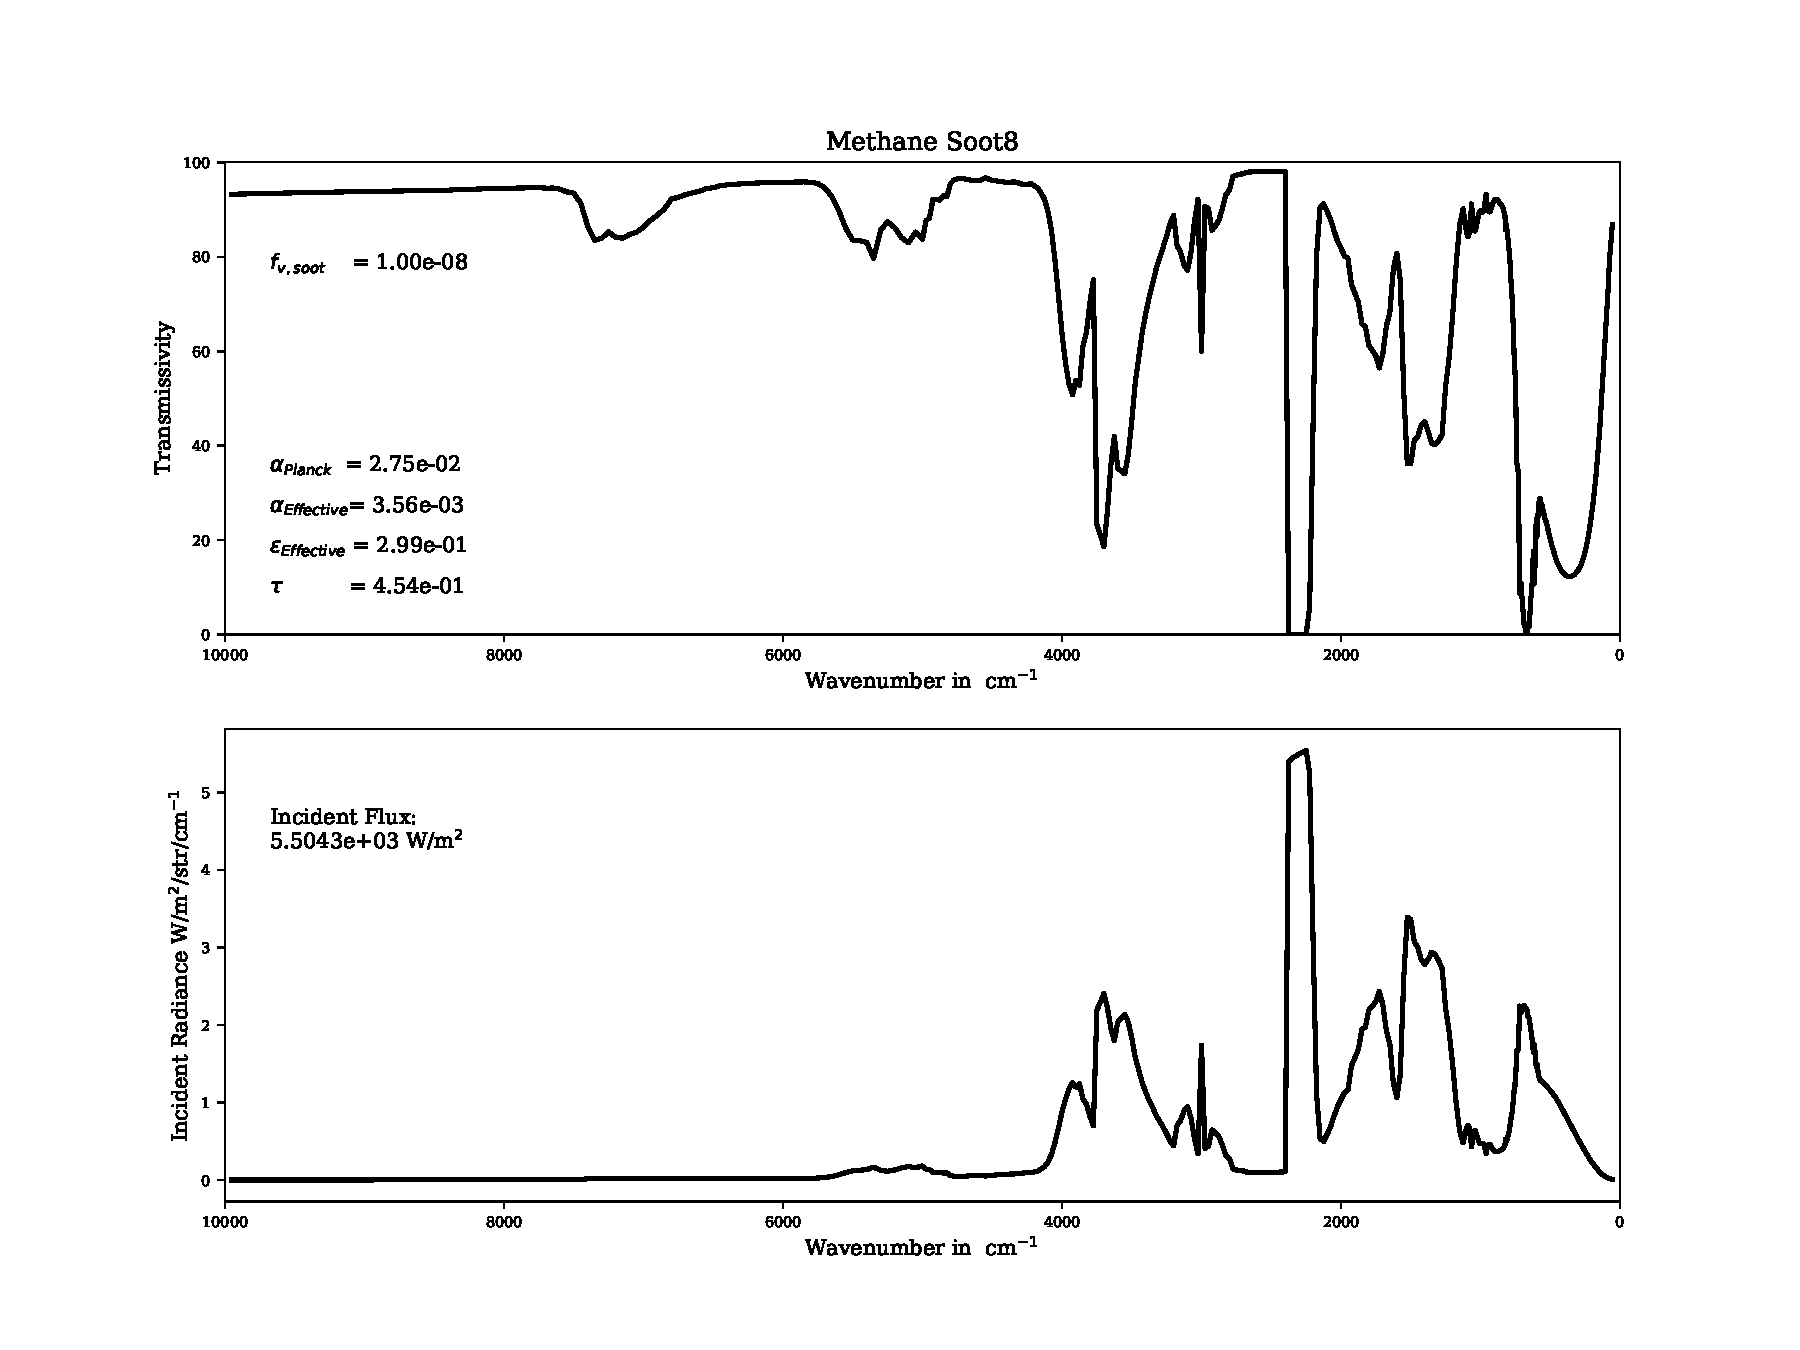
\includegraphics[width=14cm]{Figures/Cases_OriginalVersion (Soot C=7.0)/Tw300_Tg1000_Methane_1m/Methane_Soot8.pdf}%
	}
	\par\medskip		
	\centering\subfloat[The modified soot model]{%
		\centering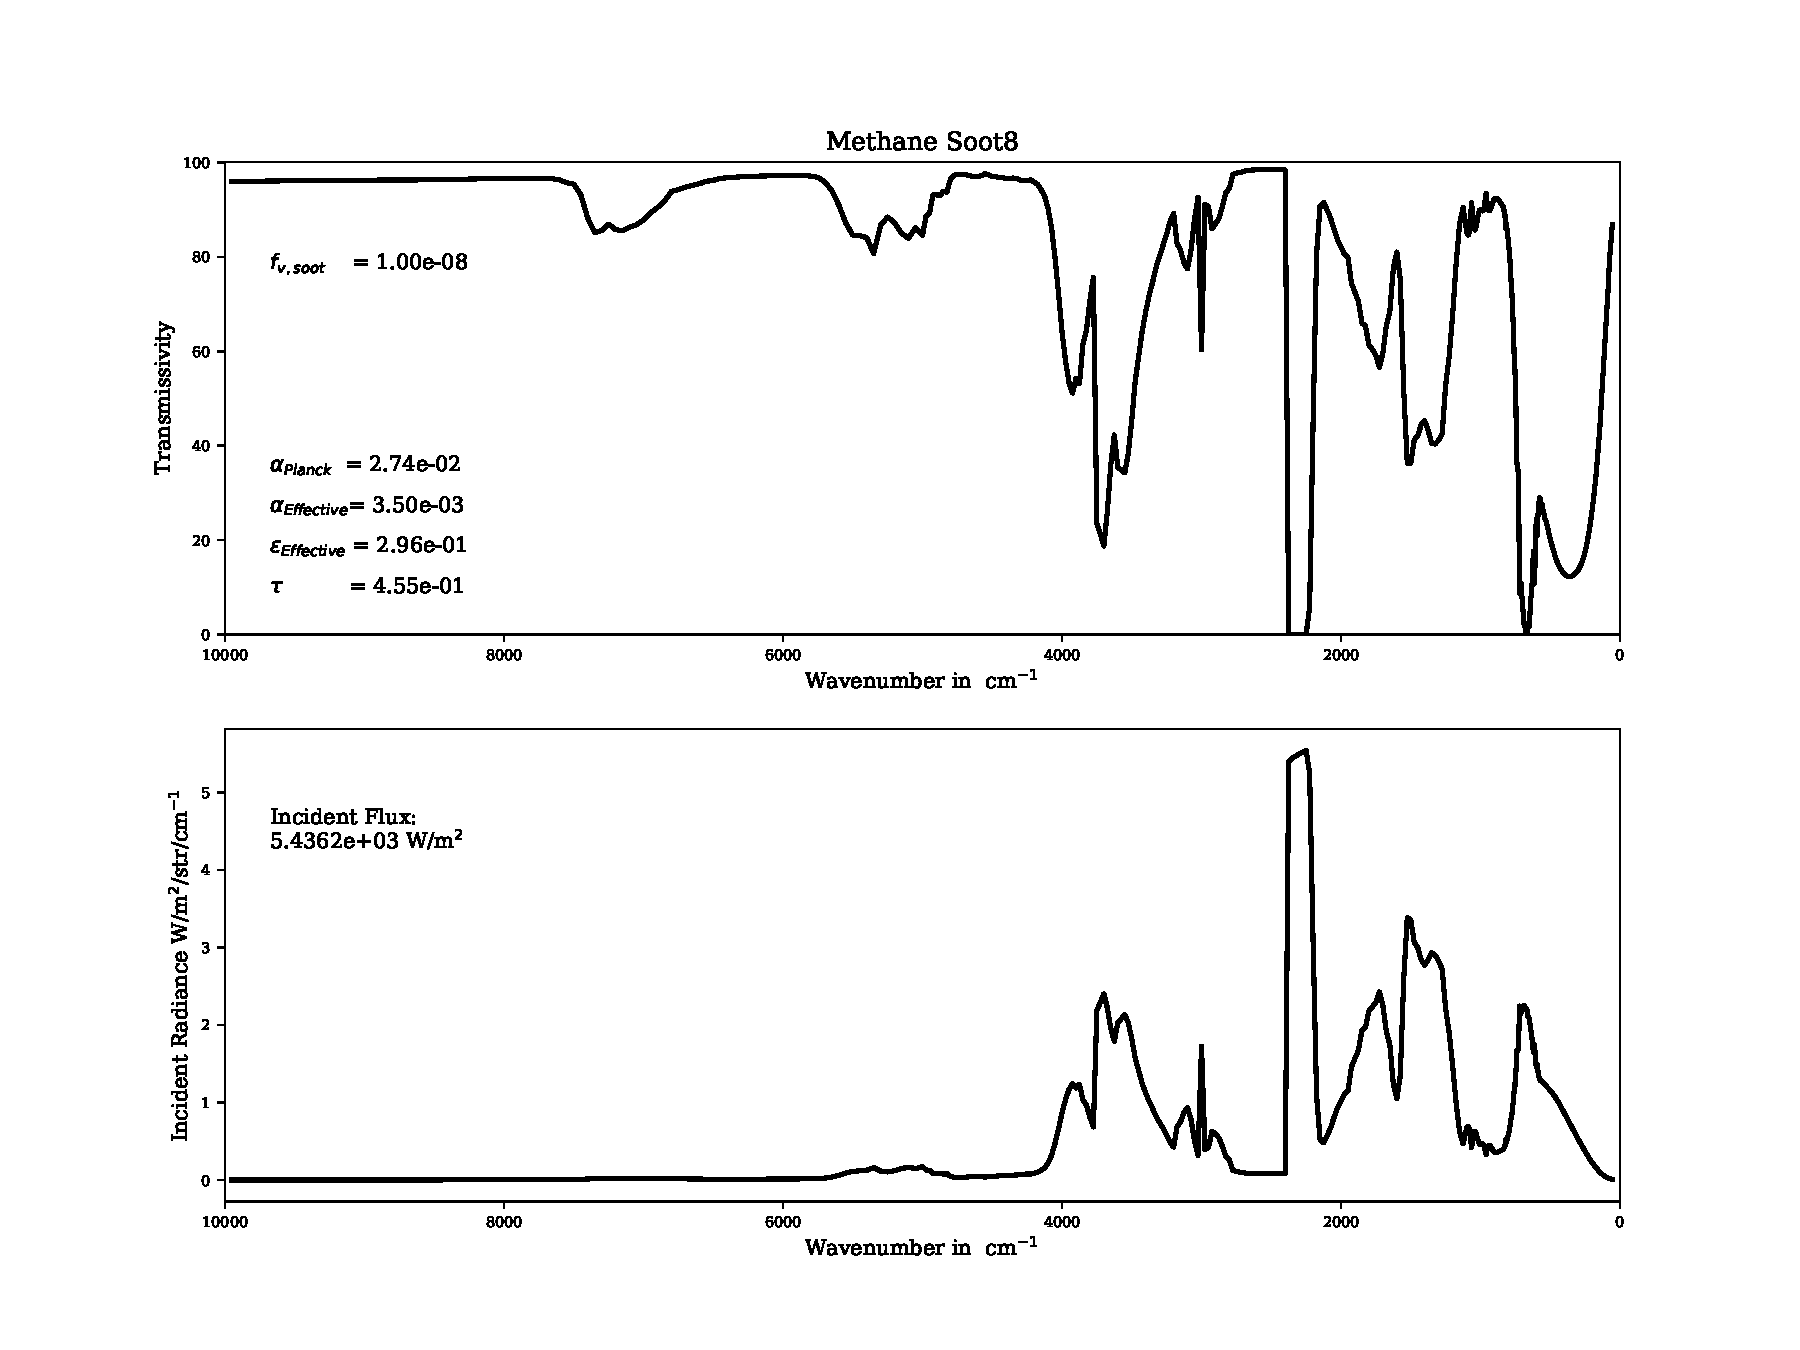
\includegraphics[width=14cm]{../Examples/Tw300_Tg1000_Methane_1m/Soot8/Methane_Soot8.pdf}%
	}
	\caption{Test case 2, \({f_v=10^{-8}}\)} \label{fig:m_s8}
\end{figure}

\begin{figure}[p]
	\centering\subfloat[The original soot model]{%
		\centering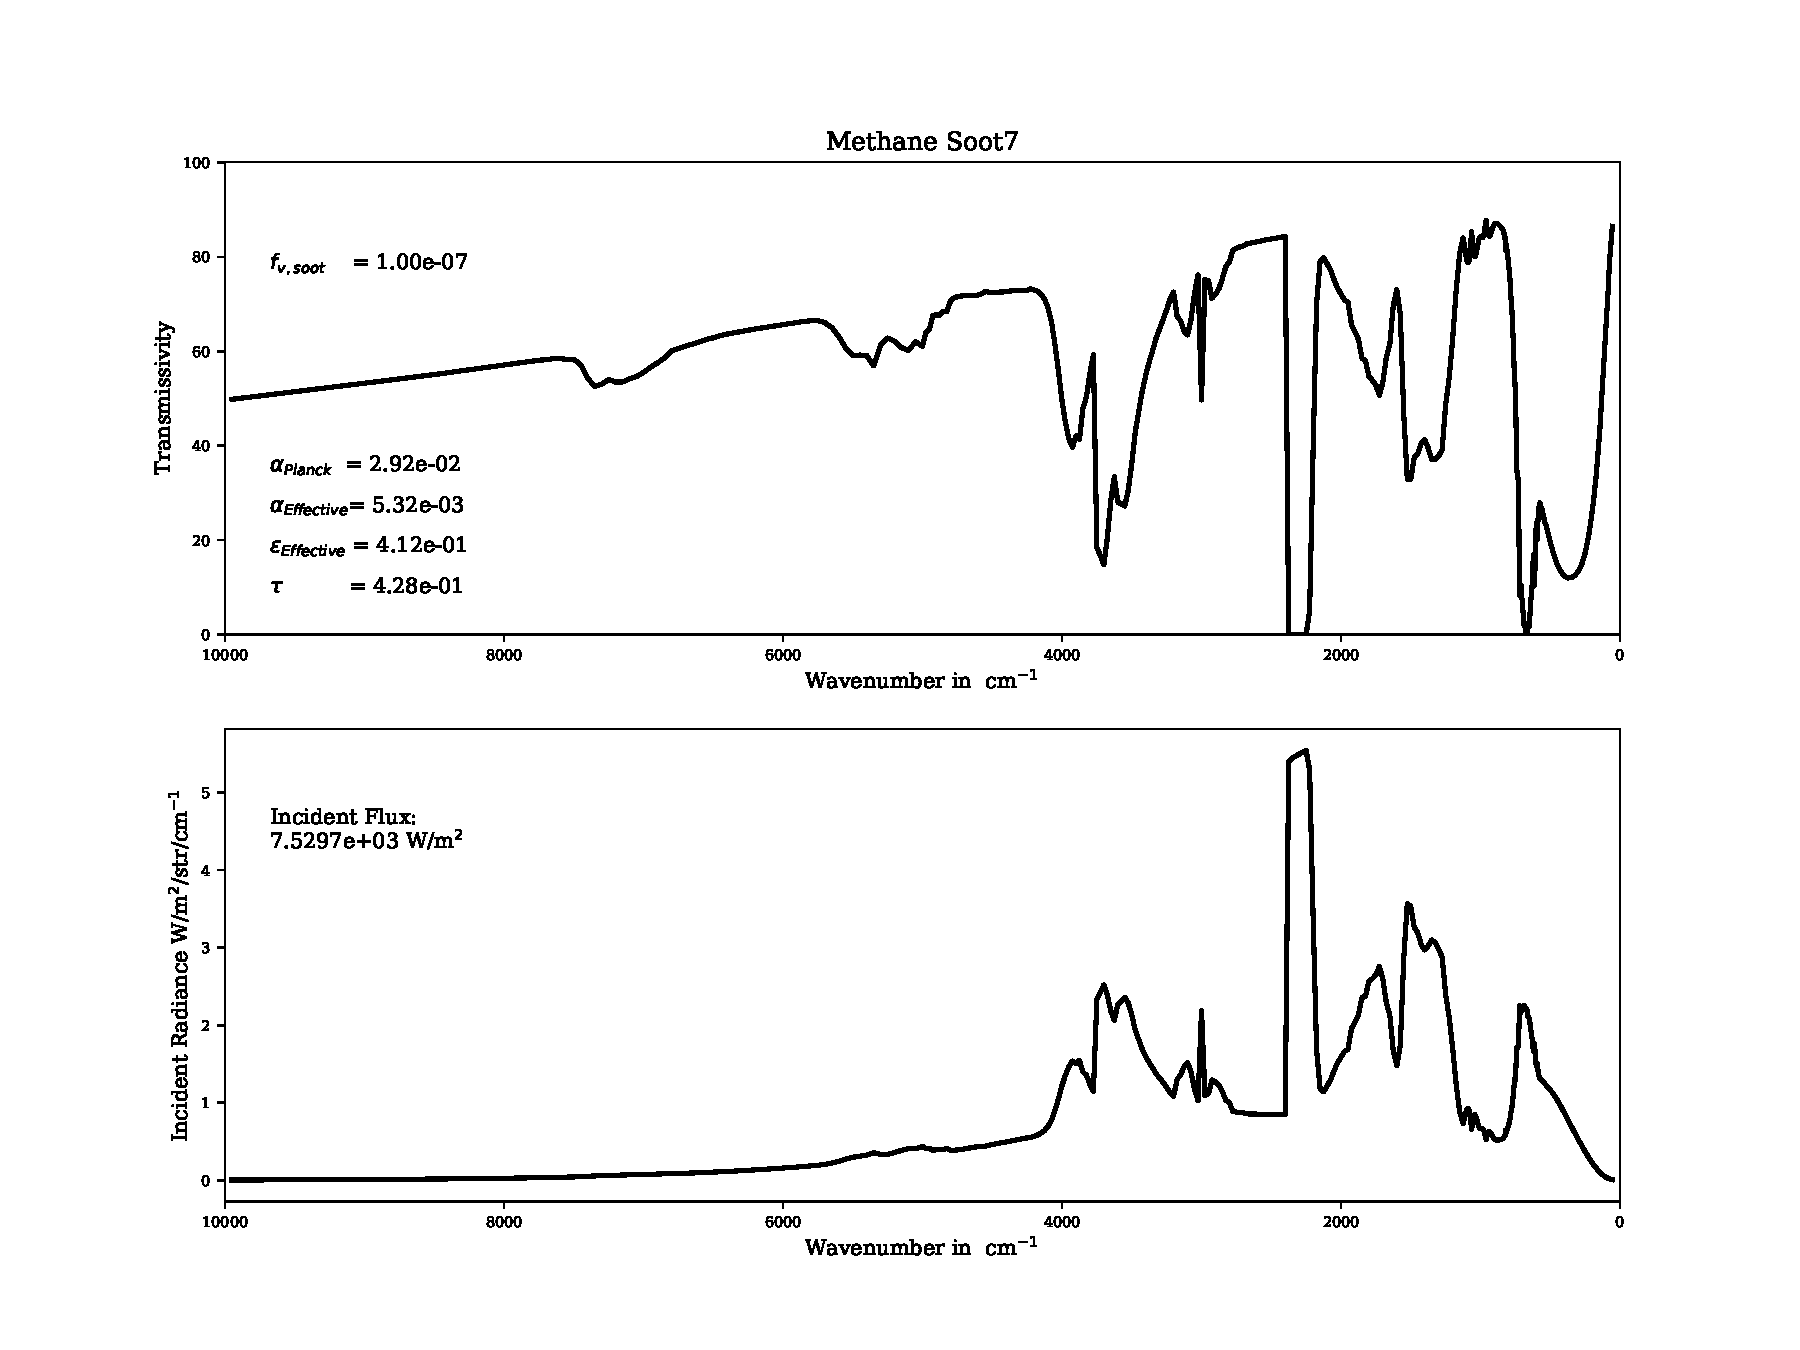
\includegraphics[width=14cm]{Figures/Cases_OriginalVersion (Soot C=7.0)/Tw300_Tg1000_Methane_1m/Methane_Soot7.pdf}%
	}
	\par\medskip		
	\centering\subfloat[The modified soot model]{%
		\centering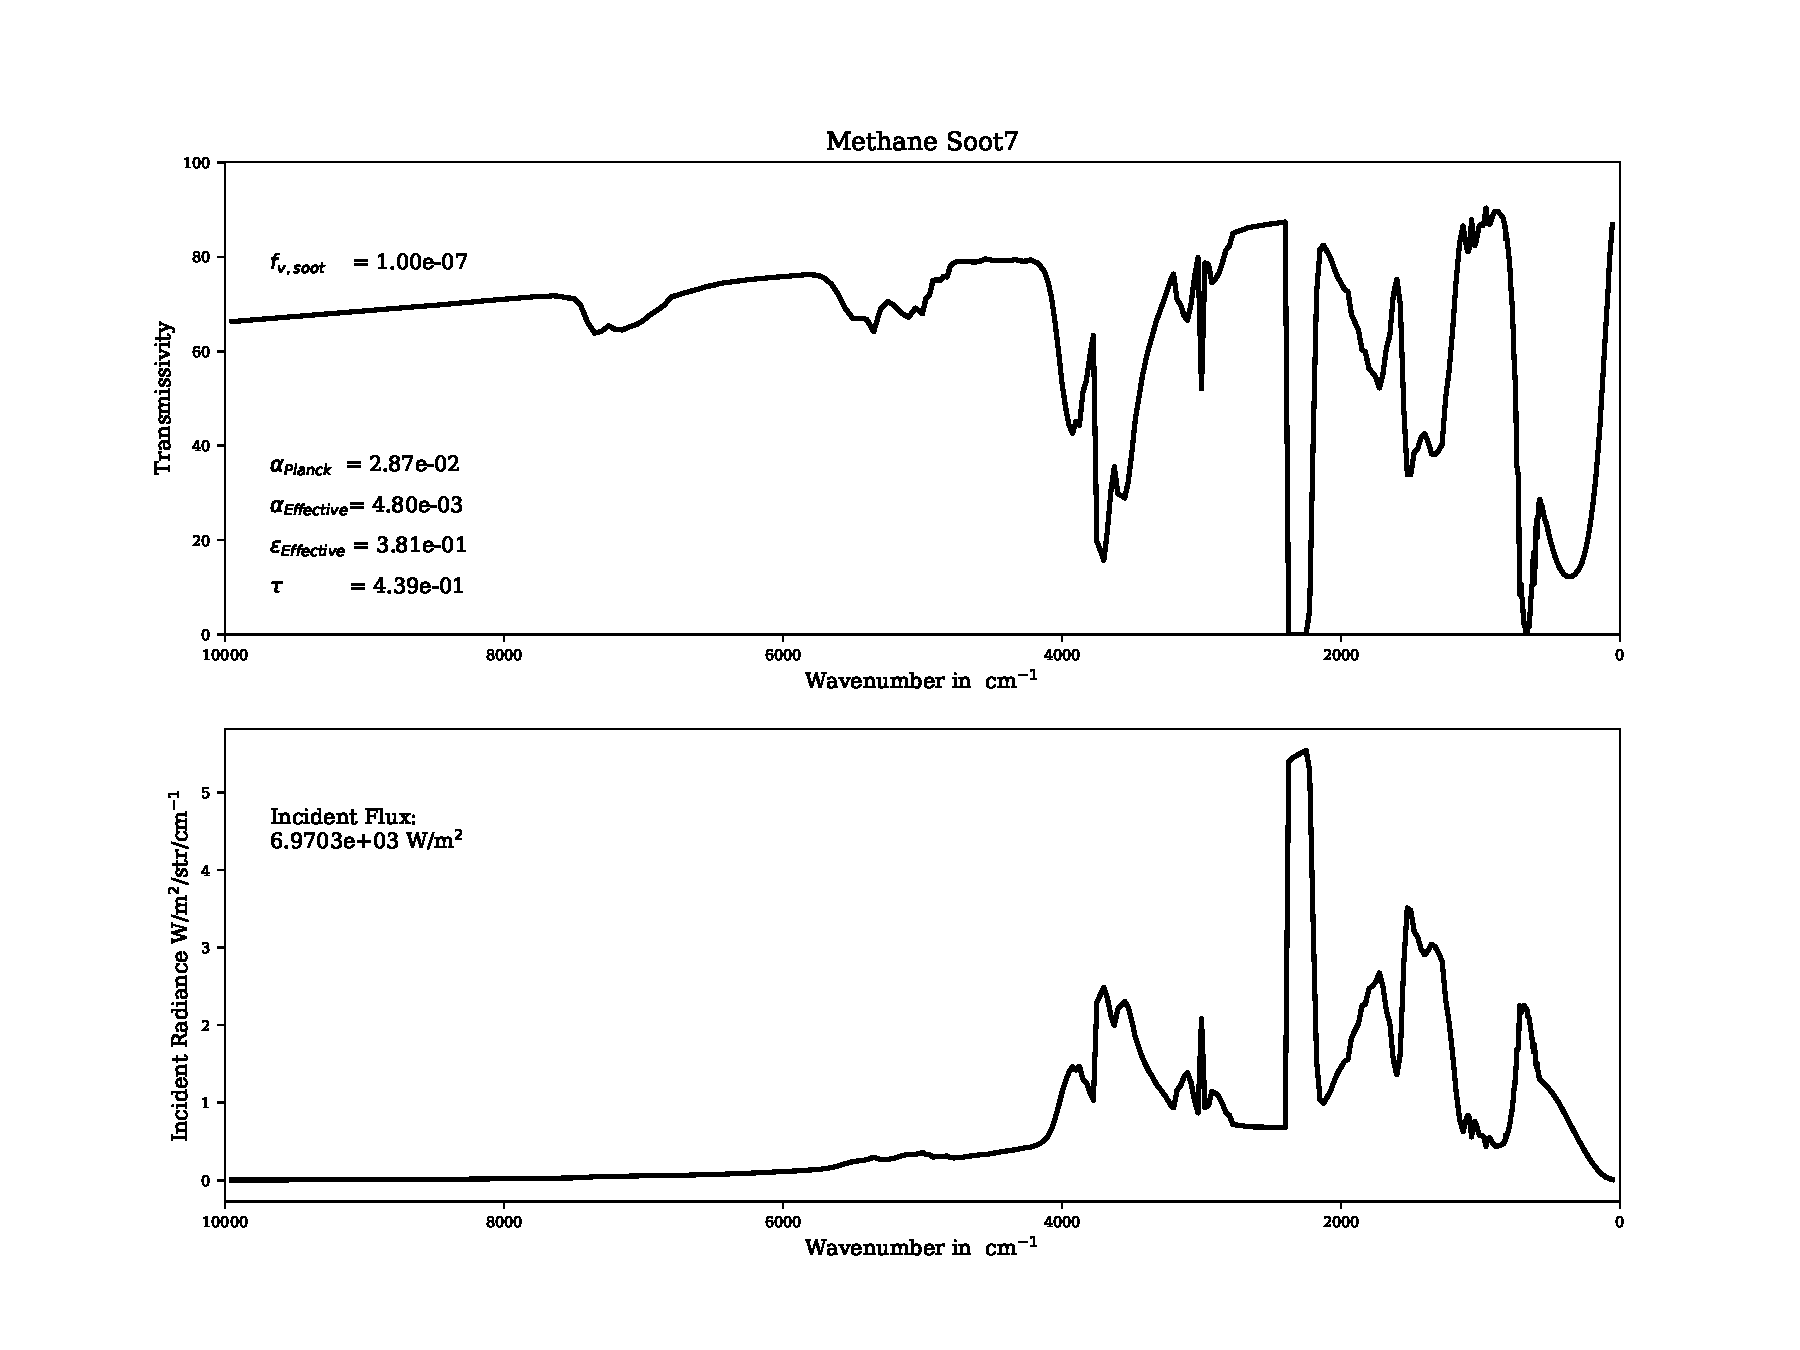
\includegraphics[width=14cm]{../Examples/Tw300_Tg1000_Methane_1m/Soot7/Methane_Soot7.pdf}%
	}
	\caption{Test case 2, \({f_v=10^{-7}}\)} \label{fig:m_s7}
\end{figure}

\pagebreak

Similarly, for the cases with very large soot concentration (e.g. \(f_{v,soot}=10^{-4}\)), the proposed modification does not alter the results. For this high level of soot load, thermal radiation is governed by emission of soot and we see that the transmissivity is almost zero in the entire spectrum. It is also inline with theoretical expectations as in this concentration level, soot blocks the radiation and the whole mixture is acting like a blackbody emitter. It is seen for instance in the intensity profile of \cref{fig:m_s4} in which \(f_{v,soot}=10^{-4}\).


\begin{figure}[p]
	\centering\subfloat[The original soot model]{%
		\centering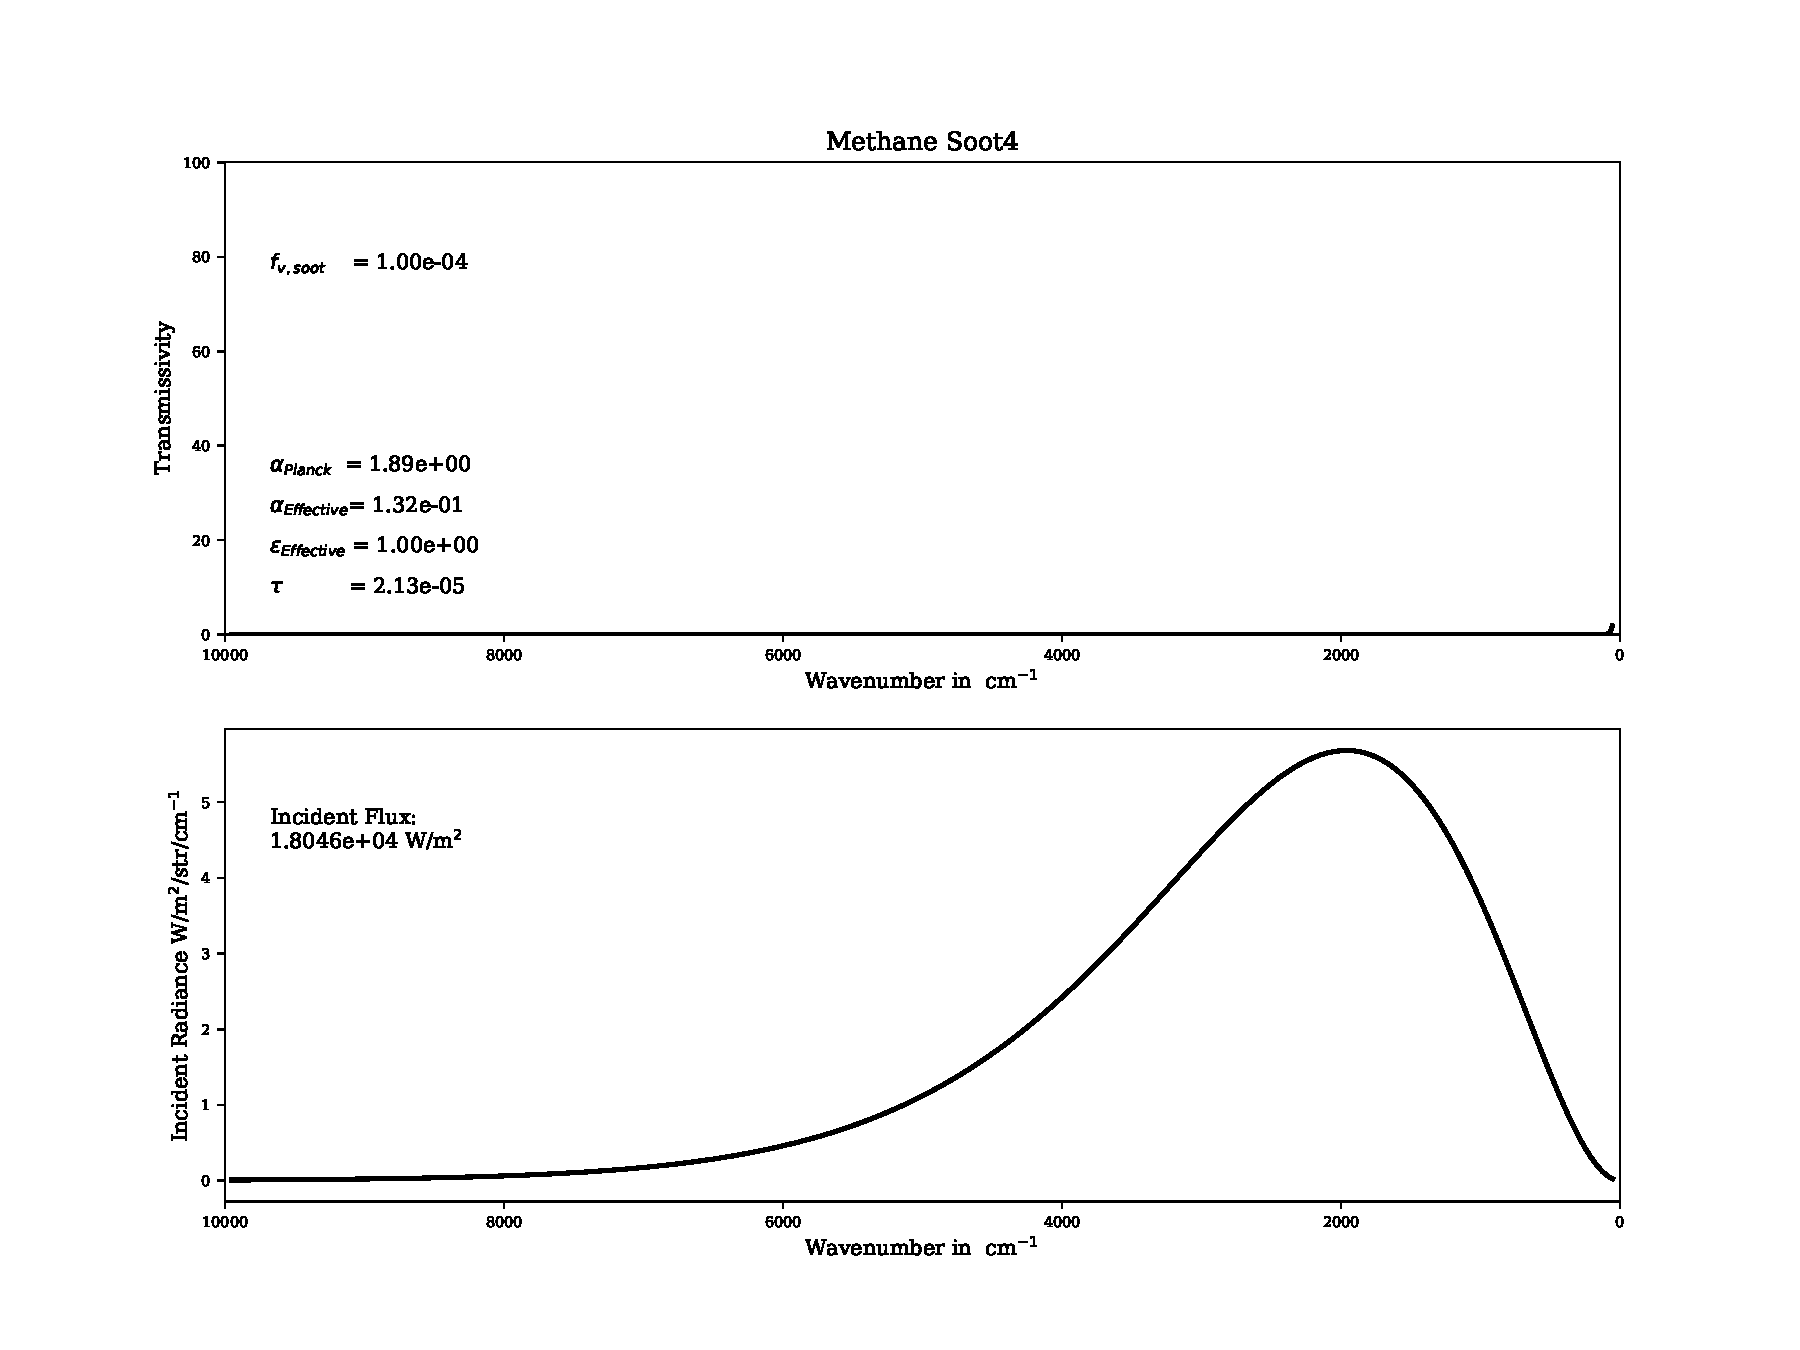
\includegraphics[width=14cm]{Figures/Cases_OriginalVersion (Soot C=7.0)/Tw300_Tg1000_Methane_1m/Methane_Soot4.pdf}%
	}
	\par\medskip		
	\centering\subfloat[The modified soot model]{%
		\centering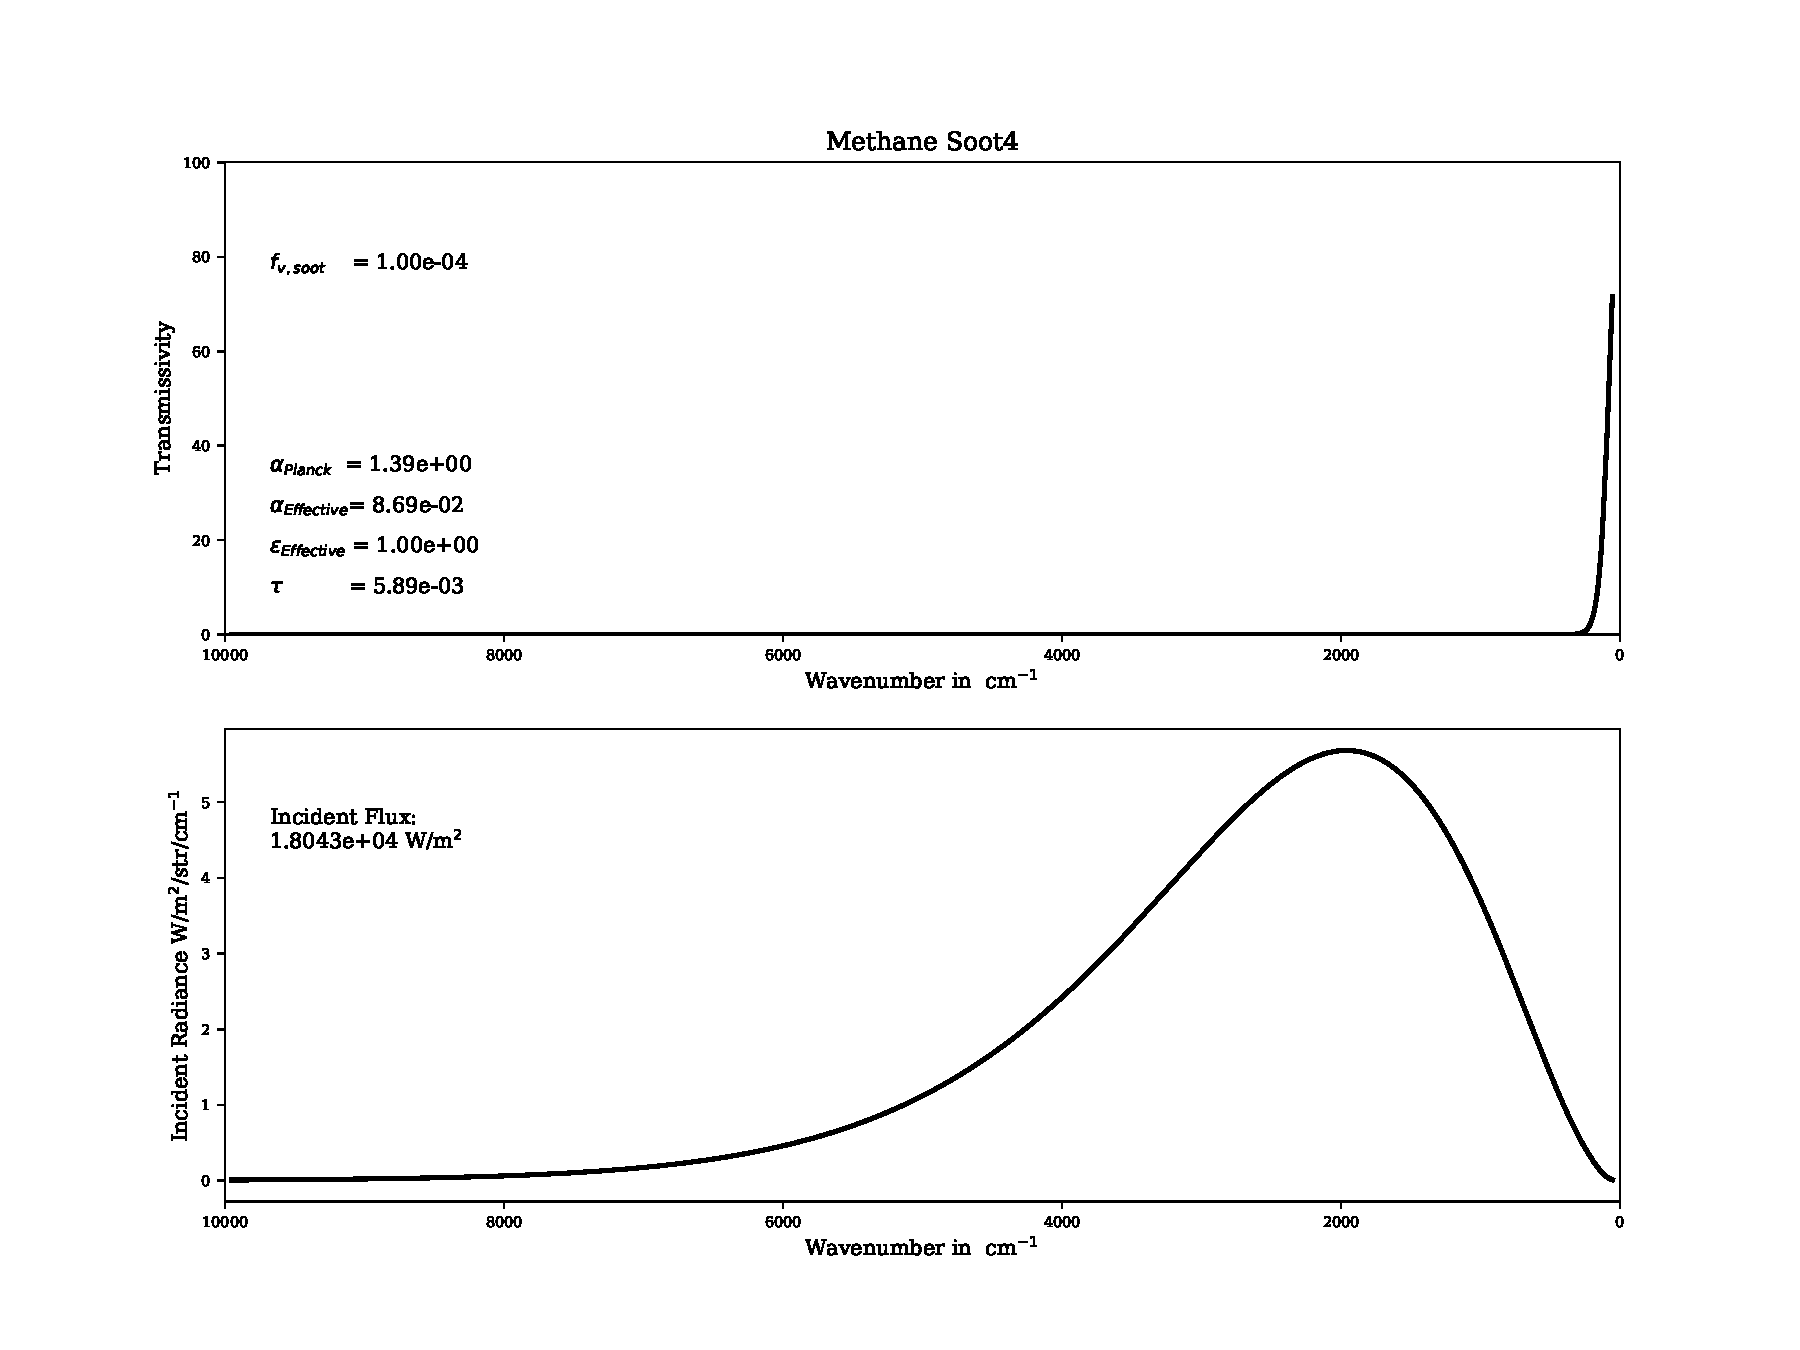
\includegraphics[width=14cm]{../Examples/Tw300_Tg1000_Methane_1m/Soot4/Methane_Soot4.pdf}%
	}
	\caption{Test case 2, \({f_v=10^{-4}}\)} \label{fig:m_s4}
\end{figure}

\pagebreak

However, for the moderate level of soot concentration (e.g. \(f_{v,soot}=10^{-5}\) and \(10^{-6}\)), quite remarkable differences are seen in predictions of two models for both profiles of transmissivity and intensity as seen in \cref{fig:m_s5,fig:m_s6}.The differences are more visible in low wavenumbers and total values.

\begin{figure}[p]
	\centering\subfloat[The original soot model]{%
		\centering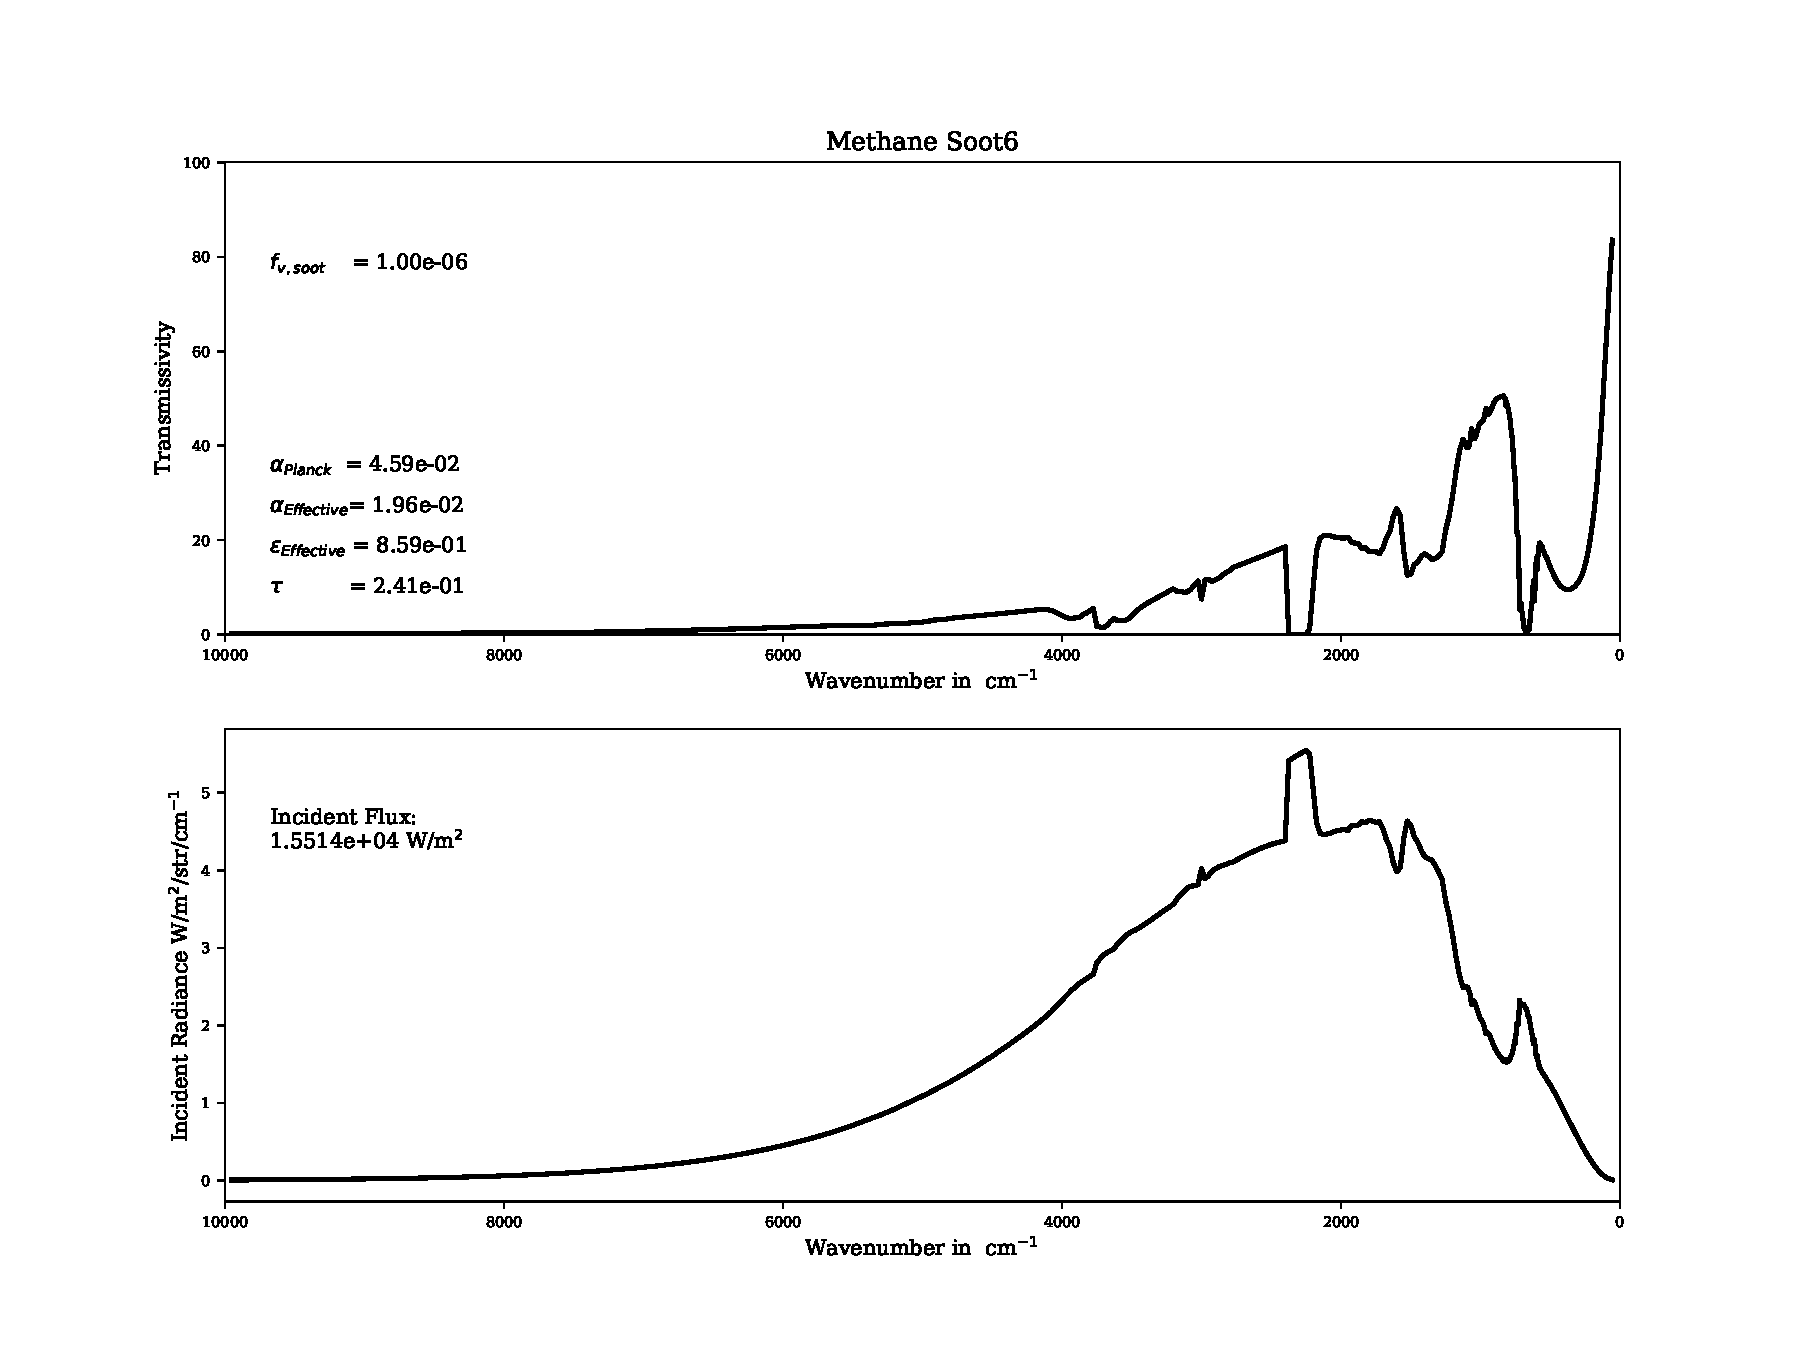
\includegraphics[width=14cm]{Figures/Cases_OriginalVersion (Soot C=7.0)/Tw300_Tg1000_Methane_1m/Methane_Soot6.pdf}%
	}
	\par\medskip		
	\centering\subfloat[The modified soot model]{%
		\centering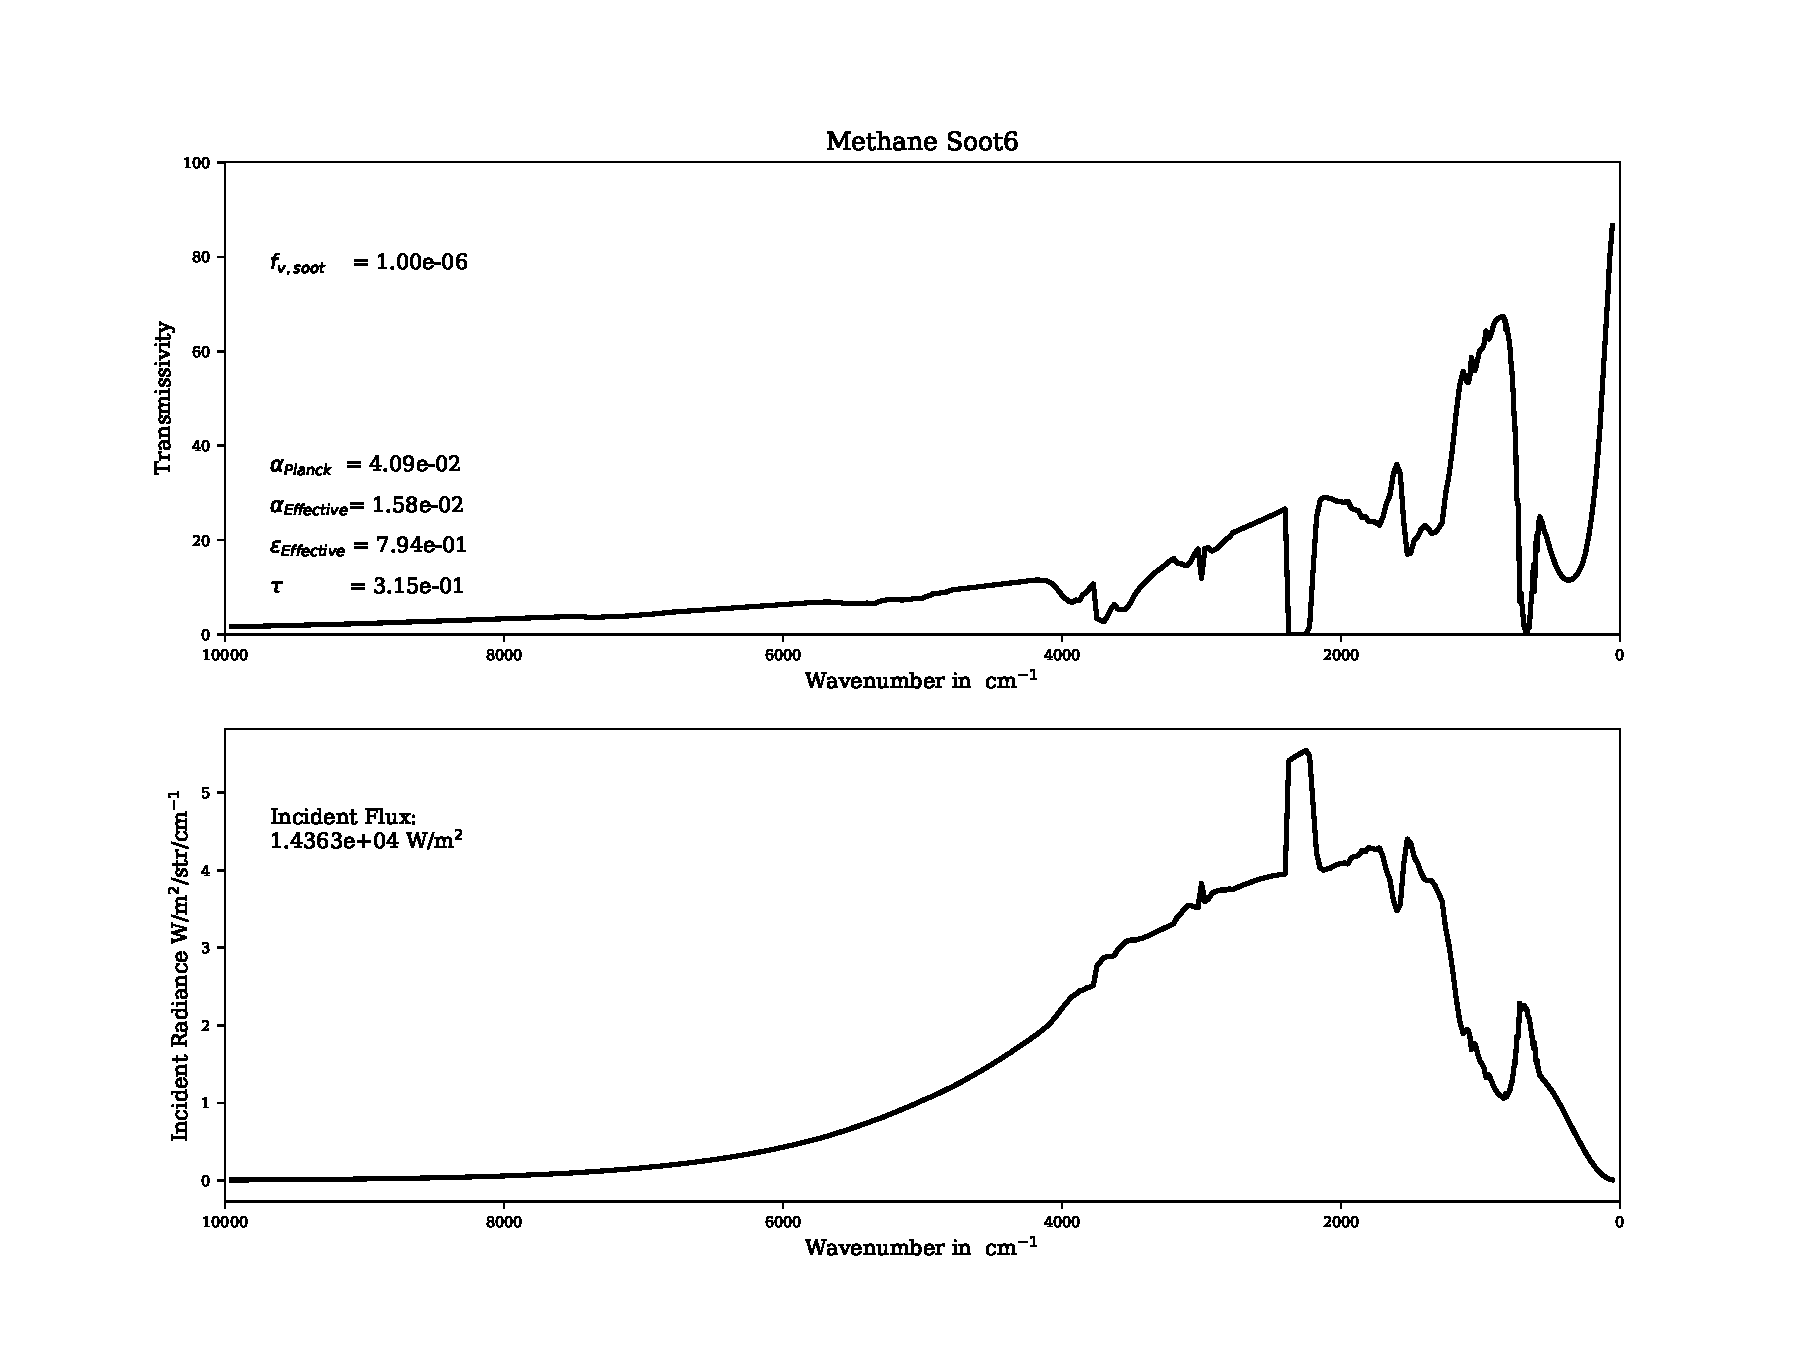
\includegraphics[width=14cm]{../Examples/Tw300_Tg1000_Methane_1m/Soot6/Methane_Soot6.pdf}%
	}
	\caption{Test case 2, \({f_v=10^{-6}}\)} \label{fig:m_s6}
\end{figure}

\begin{figure}[p]
	\centering\subfloat[The original soot model]{%
		\centering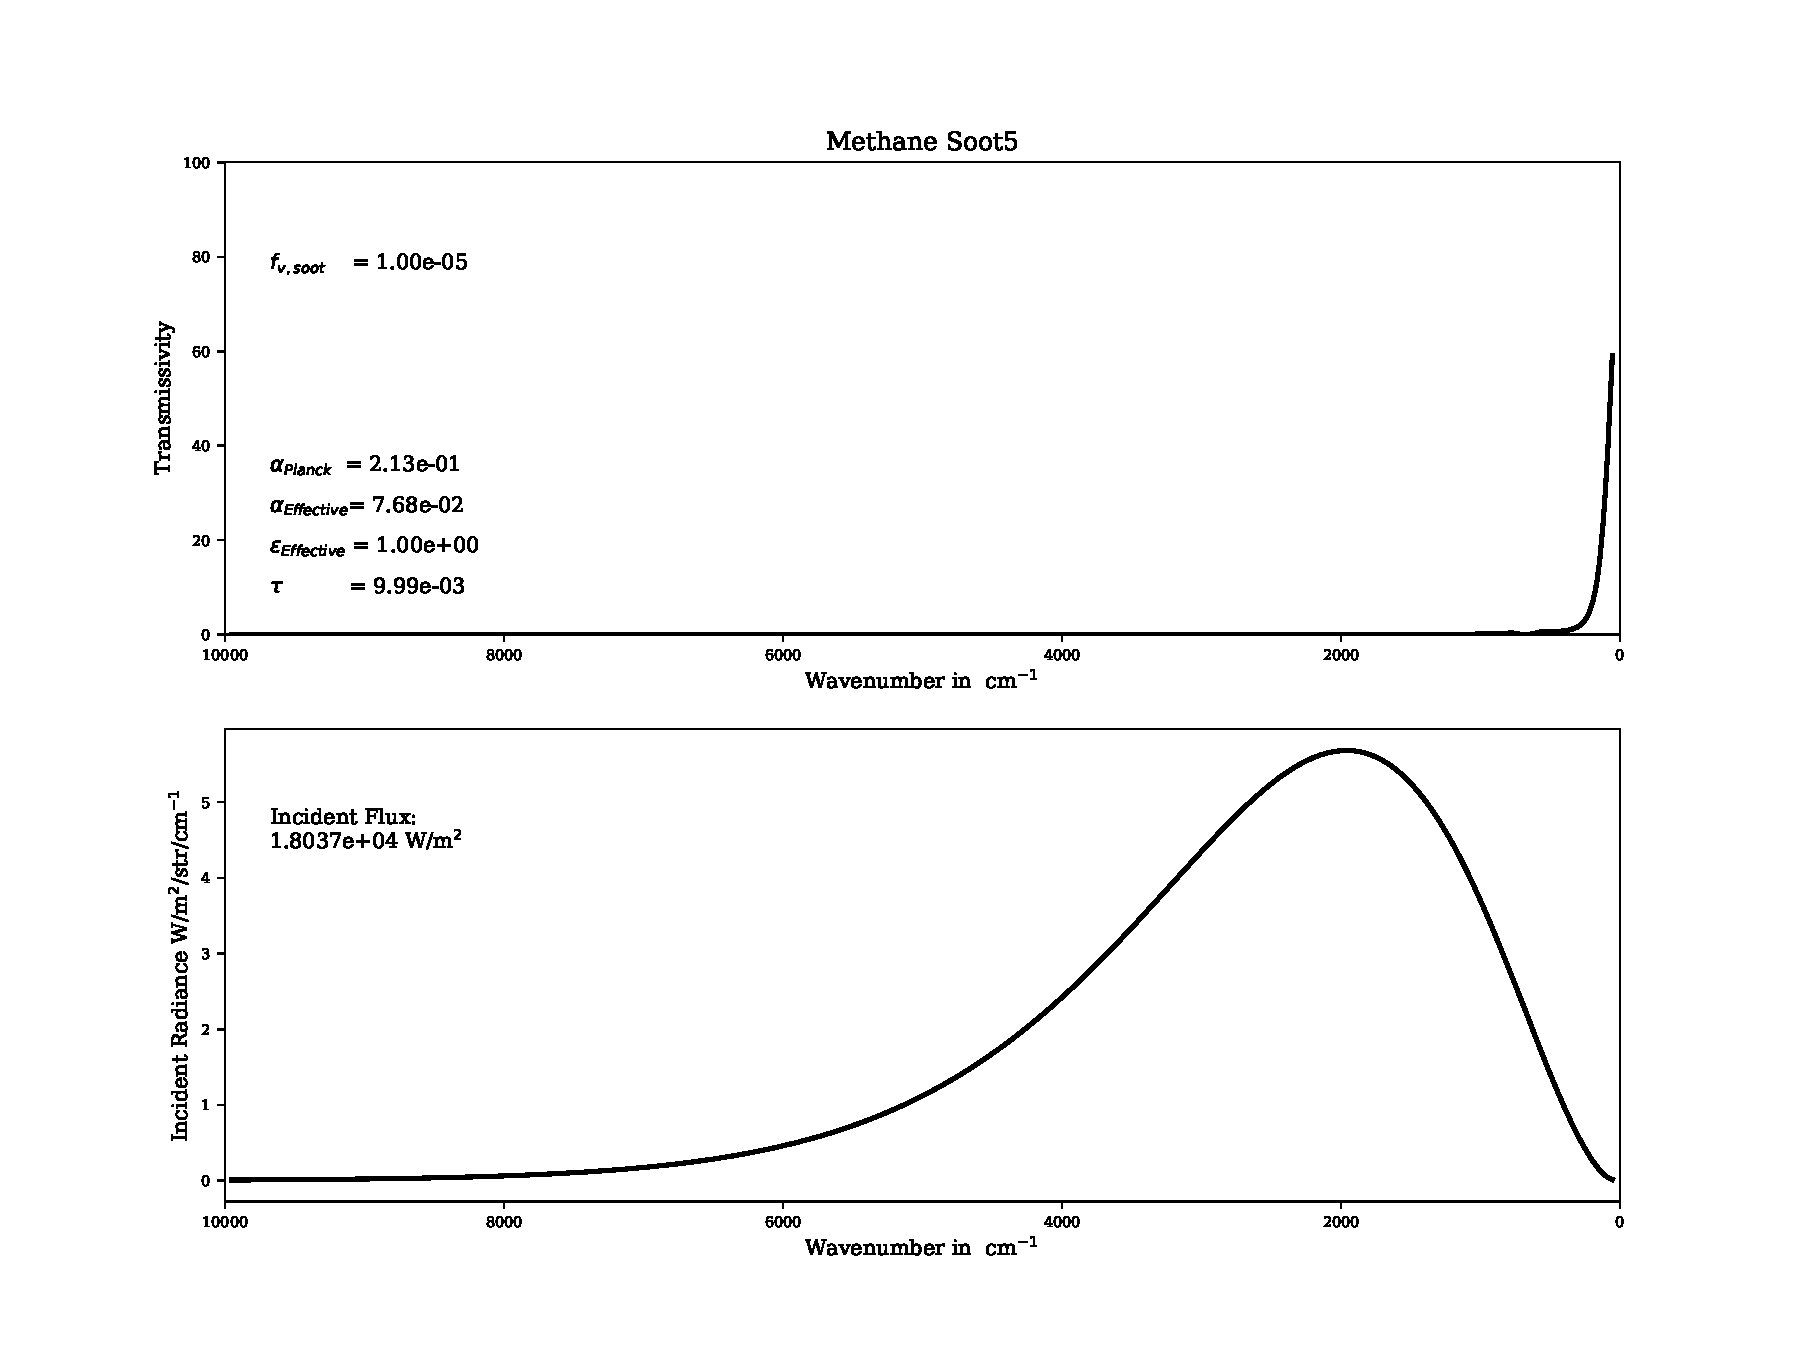
\includegraphics[width=14cm]{Figures/Cases_OriginalVersion (Soot C=7.0)/Tw300_Tg1000_Methane_1m/Methane_Soot5.pdf}%
	}
	\par\medskip		
	\centering\subfloat[The modified soot model]{%
		\centering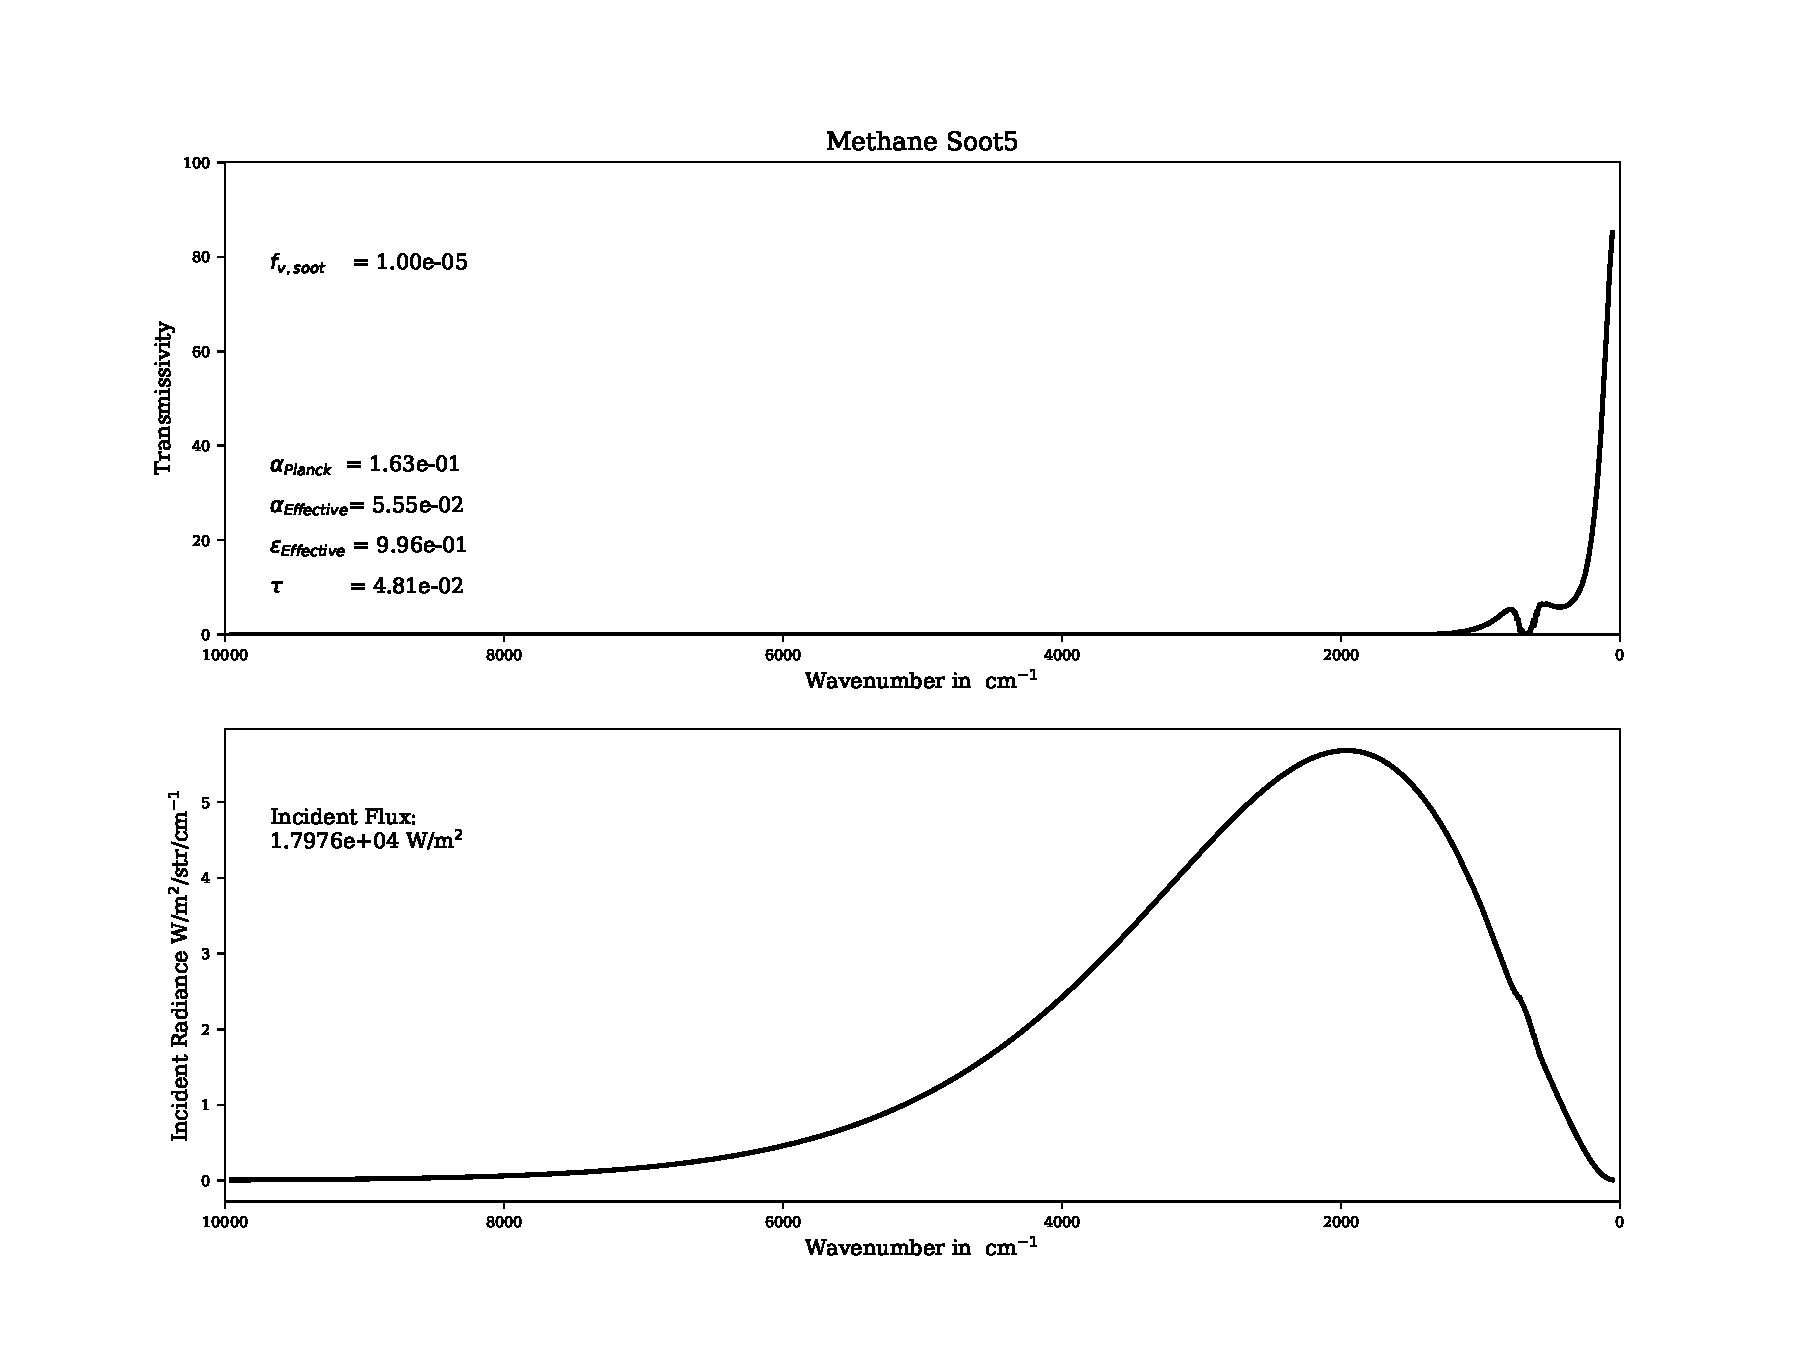
\includegraphics[width=14cm]{../Examples/Tw300_Tg1000_Methane_1m/Soot5/Methane_Soot5.pdf}%
	}
	\caption{Test case 2, \({f_v=10^{-5}}\)} \label{fig:m_s5}
\end{figure}

\pagebreak

\section{Conclusions}
A new approach to account for spectral variation of radiative properties of soot is implemented in RadCal. the new method has a better ground and is supported by a newer work of Change and Charalampopoulos \cite{ChangeCharalampopoulos1990}. Some verification cases have been tested and the clear effect of new implementation in cases with moderate soot concentration was observed.

%\section*{References}
\bibliography{mybibfile}
 
\end{document}